\documentclass[11pt,a4paper]{article}
\usepackage[margin=2.5cm]{geometry}
\usepackage{amsmath,amssymb}
\usepackage[authoryear,round]{natbib}
\usepackage{setspace}
\usepackage{graphicx}
\usepackage{booktabs}
\usepackage{float}
\onehalfspacing
\graphicspath{{figures/}}

\title{Exploratory analysis of river habitat covariates for the breeding intensity in the river-network model of onchocerciasis}
\author{}
\date{}

\begin{document}
\maketitle

\section{Purpose}

The river-network model generates the exposure of a village from breeding of blackflies along the rivers within dispersal range. Breeding currently depends on discharge and on a Gaussian field $u$ on the network. RiverATLAS \citep{linke2019} describes every reach by hydrological, physiographic and land-cover attributes, some of which plausibly govern where \textit{Simulium damnosum} s.l.\ breeds. This note explores, before fitting any model, how these attributes relate to the REMO nodule data in Sudan and South Sudan, and proposes a criterion to decide which of them enter the breeding intensity, and so the exposure $E$.

\section{From a covariate on the river to a covariate at the village}

The covariates are defined along the rivers and the outcomes at villages, and the model itself tells how the two are linked. With breeding intensity $w(s) = \exp\{\theta \log Q(s) + \beta x(s)\}$ for a covariate $x$, the exposure of village $i$ is $E_i(\beta) = \sum_j K_{ij} w_j$, where $j$ runs over the quadrature nodes of the rivers within 40~km and $K_{ij}$ is the Wendland kernel weight times the river length represented by the node. Expanding in $\beta$,
\[
\log E_i(\beta) = \log E_i(0) + \beta\, \bar{x}_i + O(\beta^2), \qquad
\bar{x}_i = \frac{\sum_j K_{ij} w_j(0)\, x_j}{\sum_j K_{ij} w_j(0)} .
\]
To first order, then, a river covariate acts on prevalence through $\bar x_i$, the average of $x$ over the rivers within reach of the village, weighted by the dispersal kernel and by breeding as it would be without the covariate. This village average can be computed without fitting anything. The main analysis takes $\theta = 0$, so that the weights are the kernel times river length; $\theta = -0.9$, the estimate of the model without $u$, is used as a check. The kernel range $\phi$ sets the scale over which rivers are averaged. The fitted models use $\phi = 40$~km, which is also the reference here, but the village averages and their associations are computed for $\phi$ = 5, 10, 20, 30, 40, 60, 80 and 100~km, to see whether the conclusions depend on it. All 900 villages have river within 40~km, but 150 have none within 5~km and 51 none within 10~km; at those ranges these villages are left out.

For each covariate a single figure shows the village averages on a map, and then two plots that follow the two parts of the zero-inflated model: the share of villages with at least one positive against the quintiles of $\bar x_i$, which relates to the probability of a zone of transmission, and the pooled prevalence among the villages with positives, which relates to the force of infection within a zone. Each plot shows all villages with 95\% Wilson intervals and, as thin lines, the same summaries within terciles of the aridity index. Aridity is already in the model and the strongest geographic gradient in the data: the dry tercile has 11 villages with positives out of 300, the middle tercile 76 and the humid tercile 263. A river covariate that only distinguishes the humid south from the dry north would look strongly associated with risk in the pooled plot and add little once aridity is accounted for. The strata lines are a direct way to see this without any model. The strength of association is summarised by Spearman correlations of $\bar x_i$ with the indicator of any positive (zone) and with the empirical logit of prevalence among villages with positives (intensity). Villages close together share rivers and risk, so ordinary intervals would be too narrow: the 95\% intervals come from a bootstrap that resamples $1^\circ \times 1^\circ$ cells (98 cells, a median of 6.5 villages per cell). Two further panels in each figure show these correlations against the kernel range, pooled with their bootstrap band and within the middle and humid terciles.

\section{Scientific rationale and expected direction}

The larvae of \textit{S.~damnosum} s.l.\ are filter feeders attached to rocks and trailing vegetation, and they need fast, turbulent, well-oxygenated water, typically at rapids, falls and spillways, and water that keeps flowing during their development \citep{crosskey1990}. This fixes the expected direction of each covariate before looking at the data. Channel slope is the closest available proxy for current speed and turbulence and should increase breeding; the share of river steeper than 2~m/km expresses the same idea as a threshold, and the velocity proxy $0.27 \log Q + 0.5 \log S$, from Manning's equation with hydraulic geometry, combines slope and discharge. Flow permanence, the ratio of the driest month's discharge to the mean, should increase breeding, since intermittent rivers interrupt larval development. Inundation, the extent of floodplain and swamp upstream, marks slow and silty water and should decrease breeding. These are the primary covariates. Hard rock, the share of river on crystalline basement or volcanic rocks in the GLiM classification \citep{hartmann2012}, provides rapids and stable substrate, and forest cover provides trailing vegetation and shade and humidity for adult flies; both should increase breeding, but forest cover upstream is also a proxy of regional climate. These are secondary. Lakes and regulation by dams have opposing effects (lake outlets and spillways are productive breeding sites, but reservoirs drown rapids, and the upstream lake percentage does not locate the outlets), and elevation and runoff have no direct mechanism beyond relief, which slope already captures, and rainfall, which aridity already captures. These have weak rationale. Discharge is already in the model and is shown for reference.

\section{Criterion for inclusion in the exposure}

A covariate is introduced in the breeding intensity, and hence in $E$, when it satisfies all of the following, judged from its figure and the summary table. First, it has a pre-specified mechanism and direction, as primary or secondary in the previous section. Second, the pooled association has the expected sign, with a block-bootstrap interval that excludes zero for at least one of the two parts. Third, the association survives aridity: in the informative strata, the middle and humid terciles (the dry tercile has only 11 villages with positives), the correlation has the expected sign with magnitude of at least 0.1 in at least one stratum and part, and is not reversed in the others. Fourth, it is robust to the scale of averaging: the second and third conditions hold for every kernel range from 20 to 80~km, the plausible span of dispersal of the vector, and with $\theta = -0.9$. Ranges of 5 and 10~km are shown but not required, as they drop villages and average over a few nodes. Fifth, it is not redundant: when two candidates have village averages correlated by more than 0.7 in absolute value, only one is kept, the one with the stronger rationale or, for equal rationale, the simpler one. The threshold of 0.1 is a judgement: with about 300 villages in a stratum it is roughly the size a correlation needs to be distinguishable from noise once spatial clustering is allowed for, and it excludes associations too small to matter for the exposure.

\section{Results}

Table~\ref{tab:eda} collects the correlations. Every covariate is associated with risk in the pooled data, most of them strongly, including elevation and runoff, which have no direct mechanism. This is the regional gradient at work: the humid south-west has steep rivers on basement rock, forest, little floodplain, higher elevation and runoff, and most of the transmission. Within aridity terciles the correlations are much smaller, typically 0.1 to 0.3, and this is where the covariates separate. The kernel range matters much less than one might expect. For most covariates the curves in panels (d) and (e) are nearly flat between 5 and 100~km, because the covariates vary smoothly in space, so that averages over 20 or over 80~km rank the villages in almost the same order. The exploration therefore cannot inform the range itself, which remains a parameter of the fitted model; it does show that the choice of covariates does not hinge on it.

\begin{table}[H]
\centering
\footnotesize\setlength{\tabcolsep}{4pt}
\caption{Spearman correlations of the village averages $\bar x_i$ (kernel range 40~km, $\theta = 0$) with the indicator of any positive (zone, 900 villages) and with the empirical logit of prevalence among villages with positives (intensity, 350 villages): pooled, with 95\% spatial block-bootstrap intervals, and within the middle and humid terciles of aridity.}
\label{tab:eda}
\begin{tabular}{llcccccc}
\toprule
 & & \multicolumn{3}{c}{Zone} & \multicolumn{3}{c}{Intensity} \\
\cmidrule(lr){3-5}\cmidrule(lr){6-8}
Covariate & Sign & Pooled & Middle & Humid & Pooled & Middle & Humid \\
\midrule
log discharge & ref. & $-0.45$ ($-0.54$, $-0.34$) & $-0.30$ & 0.12 & $-0.06$ ($-0.21$, 0.07) & $-0.13$ & 0.10 \\
log slope & $+$ & 0.37 (0.21, 0.50) & 0.04 & 0.16 & 0.31 (0.14, 0.46) & 0.28 & 0.10 \\
steep share & $+$ & 0.36 (0.20, 0.50) & 0.08 & 0.14 & 0.28 (0.12, 0.43) & 0.19 & 0.08 \\
velocity proxy & $+$ & $-0.02$ ($-0.20$, 0.14) & $-0.14$ & 0.23 & 0.26 (0.08, 0.41) & 0.17 & 0.22 \\
flow permanence & $+$ & 0.40 (0.23, 0.54) & $-0.10$ & $-0.11$ & 0.14 ($-0.05$, 0.29) & $-0.33$ & 0.06 \\
inundation & $-$ & $-0.52$ ($-0.63$, $-0.39$) & $-0.07$ & $-0.16$ & $-0.40$ ($-0.54$, $-0.24$) & $-0.21$ & $-0.18$ \\
hard rock & $+$ & 0.40 (0.23, 0.54) & 0.04 & 0.22 & 0.39 (0.23, 0.52) & 0.25 & 0.21 \\
forest & $+$ & 0.45 (0.31, 0.58) & 0.01 & 0.22 & 0.42 (0.26, 0.55) & 0.06 & 0.31 \\
lakes & ? & $-0.39$ ($-0.51$, $-0.24$) & $-0.06$ & $-0.01$ & $-0.22$ ($-0.40$, $-0.03$) & $-0.14$ & $-0.03$ \\
regulation & ? & $-0.46$ ($-0.57$, $-0.34$) & $-0.10$ & $-0.03$ & $-0.28$ ($-0.39$, $-0.17$) & $-0.17$ & $-0.09$ \\
elevation & none & 0.50 (0.36, 0.62) & 0.08 & 0.12 & 0.33 (0.14, 0.50) & 0.19 & 0.09 \\
runoff & none & 0.51 (0.36, 0.63) & 0.18 & 0.21 & 0.20 (0.06, 0.34) & $-0.14$ & 0.12 \\
\bottomrule
\end{tabular}
\end{table}

Channel slope (Figure~\ref{fig:slope}) satisfies every condition. The share of villages with positives rises from about 25\% in the three lowest quintiles to 80\% in the highest, and prevalence among villages with positives rises from 11\% to 25\%. Much of the rise in the zone plot is the step from dry to humid villages, but within strata the association remains positive: 0.16 for the zone in the humid tercile and 0.28 for intensity in the middle tercile. The pooled correlations stay at 0.36--0.37 for the zone and 0.31--0.33 for intensity at every range; within the middle tercile the intensity correlation rises from 0.12 at 20~km to 0.26--0.35 from 30~km upwards, and within the humid tercile the zone correlation lies between 0.15 and 0.19 from 10~km. The share of steep river is correlated 0.89 with log slope and tells the same story; being redundant, it is dropped in favour of the continuous measure. The velocity proxy (Figure~\ref{fig:velocity}) does not meet the criterion in its own right, since its pooled zone correlation changes sign with the kernel range, from $-0.19$ at 5~km to $-0.14$ at 20~km, 0.03 at 60~km and 0.09 at 100~km, and its zone correlation in the middle tercile is reversed ($-0.21$ to $-0.06$ between 20 and 80~km); in any case, with $\log Q$ already in the breeding intensity, a term in log velocity is the same model as a term in log slope, so it brings nothing new.

Flow permanence (Figure~\ref{fig:permanence}) has a strong pooled zone correlation, 0.40, but it reverses within strata ($-0.10$ and $-0.11$ for the zone, $-0.33$ for intensity in the middle tercile). Its pooled association is the north--south rainfall gradient rather than a habitat effect, and it fails the third condition at every kernel range. Inundation (Figure~\ref{fig:inundation}) satisfies all conditions with the expected negative sign: $-0.52$ and $-0.40$ pooled, and between $-0.07$ and $-0.21$ within strata, consistently negative for kernel ranges from 20 to 80~km, although in the middle tercile the zone correlation is small ($-0.02$ to $-0.08$) and the condition is met through the humid tercile and the intensity part. Its correlation with log slope is $-0.63$, high but below the redundancy threshold, as one expects of two sides of the same contrast between steep and flat river.

Hard rock (Figure~\ref{fig:hardrock}) satisfies all conditions, with within-stratum correlations of 0.22 for the zone in the humid tercile and 0.25 and 0.21 for intensity at 40~km, and humid-tercile correlations of 0.20--0.25 at every range; it is correlated 0.66 with log slope. Forest cover (Figure~\ref{fig:forest}) satisfies the conditions through the humid tercile (0.22 for the zone, 0.31 for intensity), with essentially no association in the middle tercile, which fits forest acting where it exists, in the humid south-west, but leaves open that forest stands in for unmeasured humid conditions there. The kernel range reinforces this doubt: forest is the one candidate whose association grows steadily with the range, pooled from 0.32 at 5~km to 0.58 at 100~km for the zone, and in the middle tercile from $-0.10$ to 0.21. A habitat effect should be strongest for the rivers nearest the village; an association that strengthens as more distant river is averaged in is what a regional marker of the forested south-west would produce. Forest meets the formal criterion through the humid tercile at all ranges, but it is the weakest of the candidates.

Lakes and regulation (Figures~\ref{fig:lakes} and \ref{fig:regulation}) are negatively associated in the pooled data, because lakes and dams lie mainly on the large rivers, which dominate the river within reach in the drier north, and their correlations fall to near zero within strata; with weak rationale and an expected direction that cannot be fixed, they are excluded. Elevation and runoff (Figures~\ref{fig:elevation} and \ref{fig:runoff}) are the most strongly associated covariates in the pooled data. Elevation falls to about 0.1 within strata. Runoff is different: it keeps a correlation of about 0.2 with the zone in both the middle and the humid tercile at every range, but it reverses for intensity in the middle tercile ($-0.14$). Both are excluded by the first condition, since neither has a mechanism of its own; runoff is, however, the one excluded covariate with a consistent within-stratum signal, and as a measure of how wet the catchment is it may carry information on flow permanence in small streams that the modelled discharge ratio misses. It could be reconsidered as an alternative to flow permanence if there is a case for it on biological grounds. Discharge (Figure~\ref{fig:discharge}) shows fewer villages with positives where the rivers within reach are larger, $-0.45$ pooled and $-0.30$ in the middle tercile, consistent with the negative coefficient of $\log Q$ in the fitted models.

By the criterion, four covariates enter the breeding intensity: log channel slope and inundation as primary covariates, hard rock and forest cover as secondary ones. Their village averages are moderately correlated (slope with hard rock 0.66, slope with inundation $-0.63$, forest with the others at most 0.31), so a joint model will apportion their effects with some imprecision. A sensible order is to add slope and inundation first, then hard rock and forest, and to compare each step by marginal likelihood and cross-validation.

\section{Limits of the exploration}

The correlations are unadjusted apart from the stratification by aridity, and terciles of aridity remove only part of the regional gradient; the decision for the secondary covariates in particular rests on associations of 0.2 to 0.3 within a single stratum. The first-order expansion that justifies the village average holds for moderate effects; a covariate whose effect works through a few highly suitable sites, such as rapids, would be better described by a threshold summary, which the steep share approximates. The stratified correlations carry no intervals, and in the humid tercile the zone part rests on only 37 villages without positives. These limits are the reason the final decision belongs to the fitted model with the field $u$, which accounts for the remaining spatial structure, and to cross-validation.

\section*{Figures}

\begin{figure}[H]\centering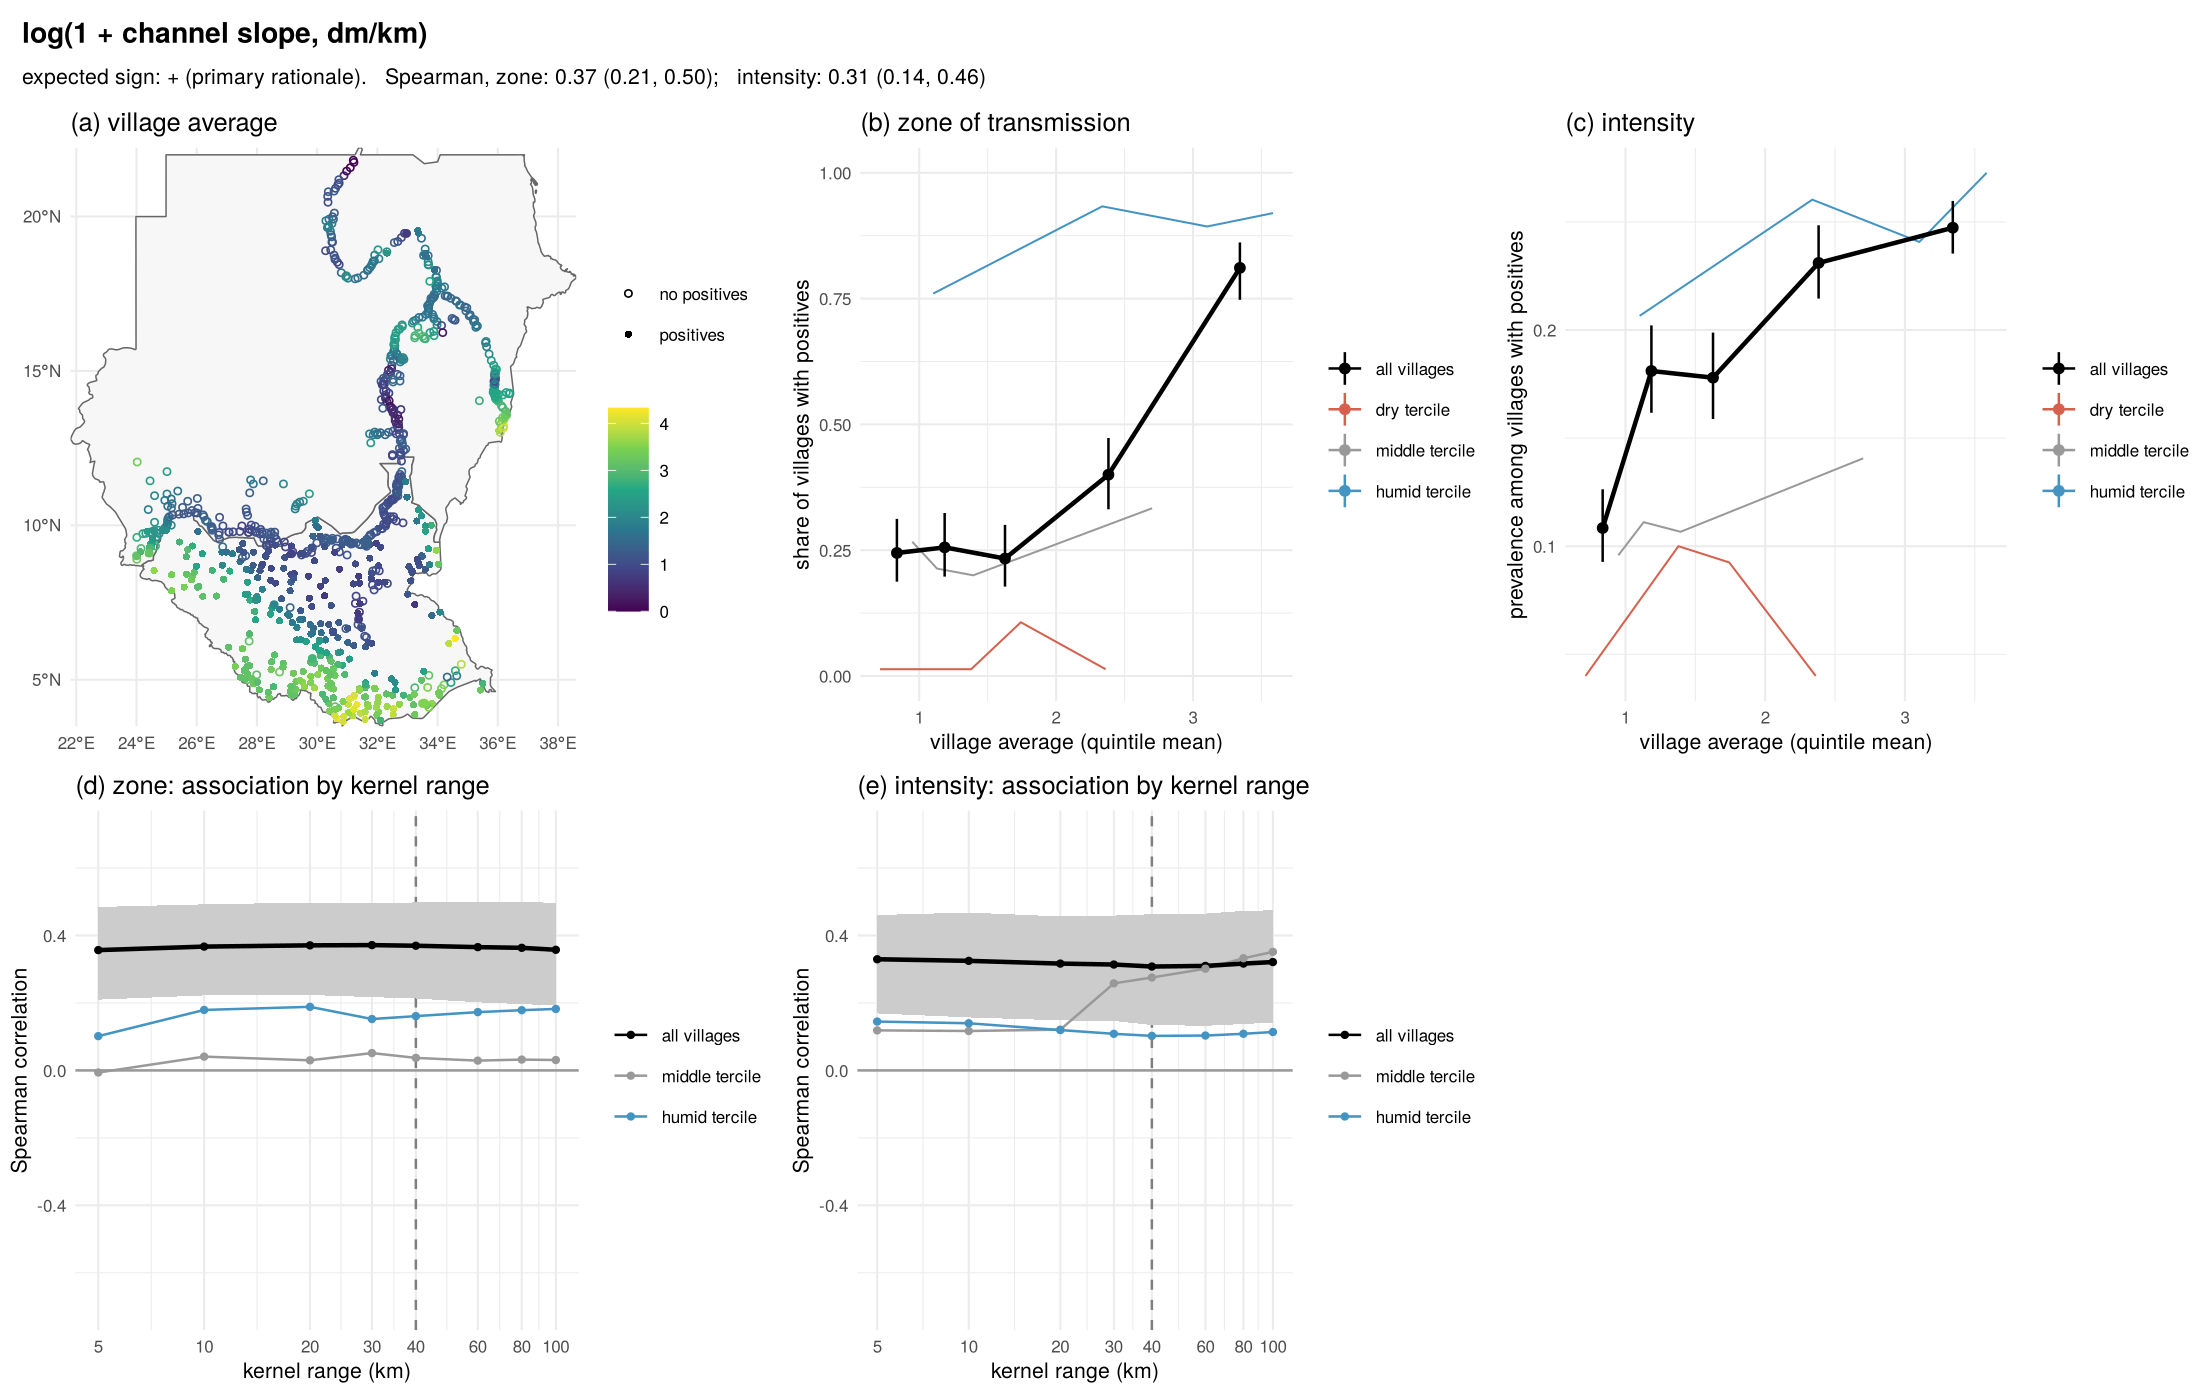
\includegraphics[width=\textwidth]{eda_log_slope.png}
\caption{Channel slope. (a) Village average of $\log(1 + \text{slope})$ within 40~km; open circles are villages without positives. (b) Share of villages with at least one positive and (c) prevalence among villages with positives, by quintile of the village average, with 95\% Wilson intervals (black), and by quartile within terciles of aridity (thin lines). (d) Spearman correlation with the indicator of any positive and (e) with the empirical logit among villages with positives, against the kernel range: pooled with 95\% spatial block-bootstrap band, and within the middle and humid terciles of aridity; the dashed line marks the 40~km range of the fitted models.}\label{fig:slope}\end{figure}
\begin{figure}[H]\centering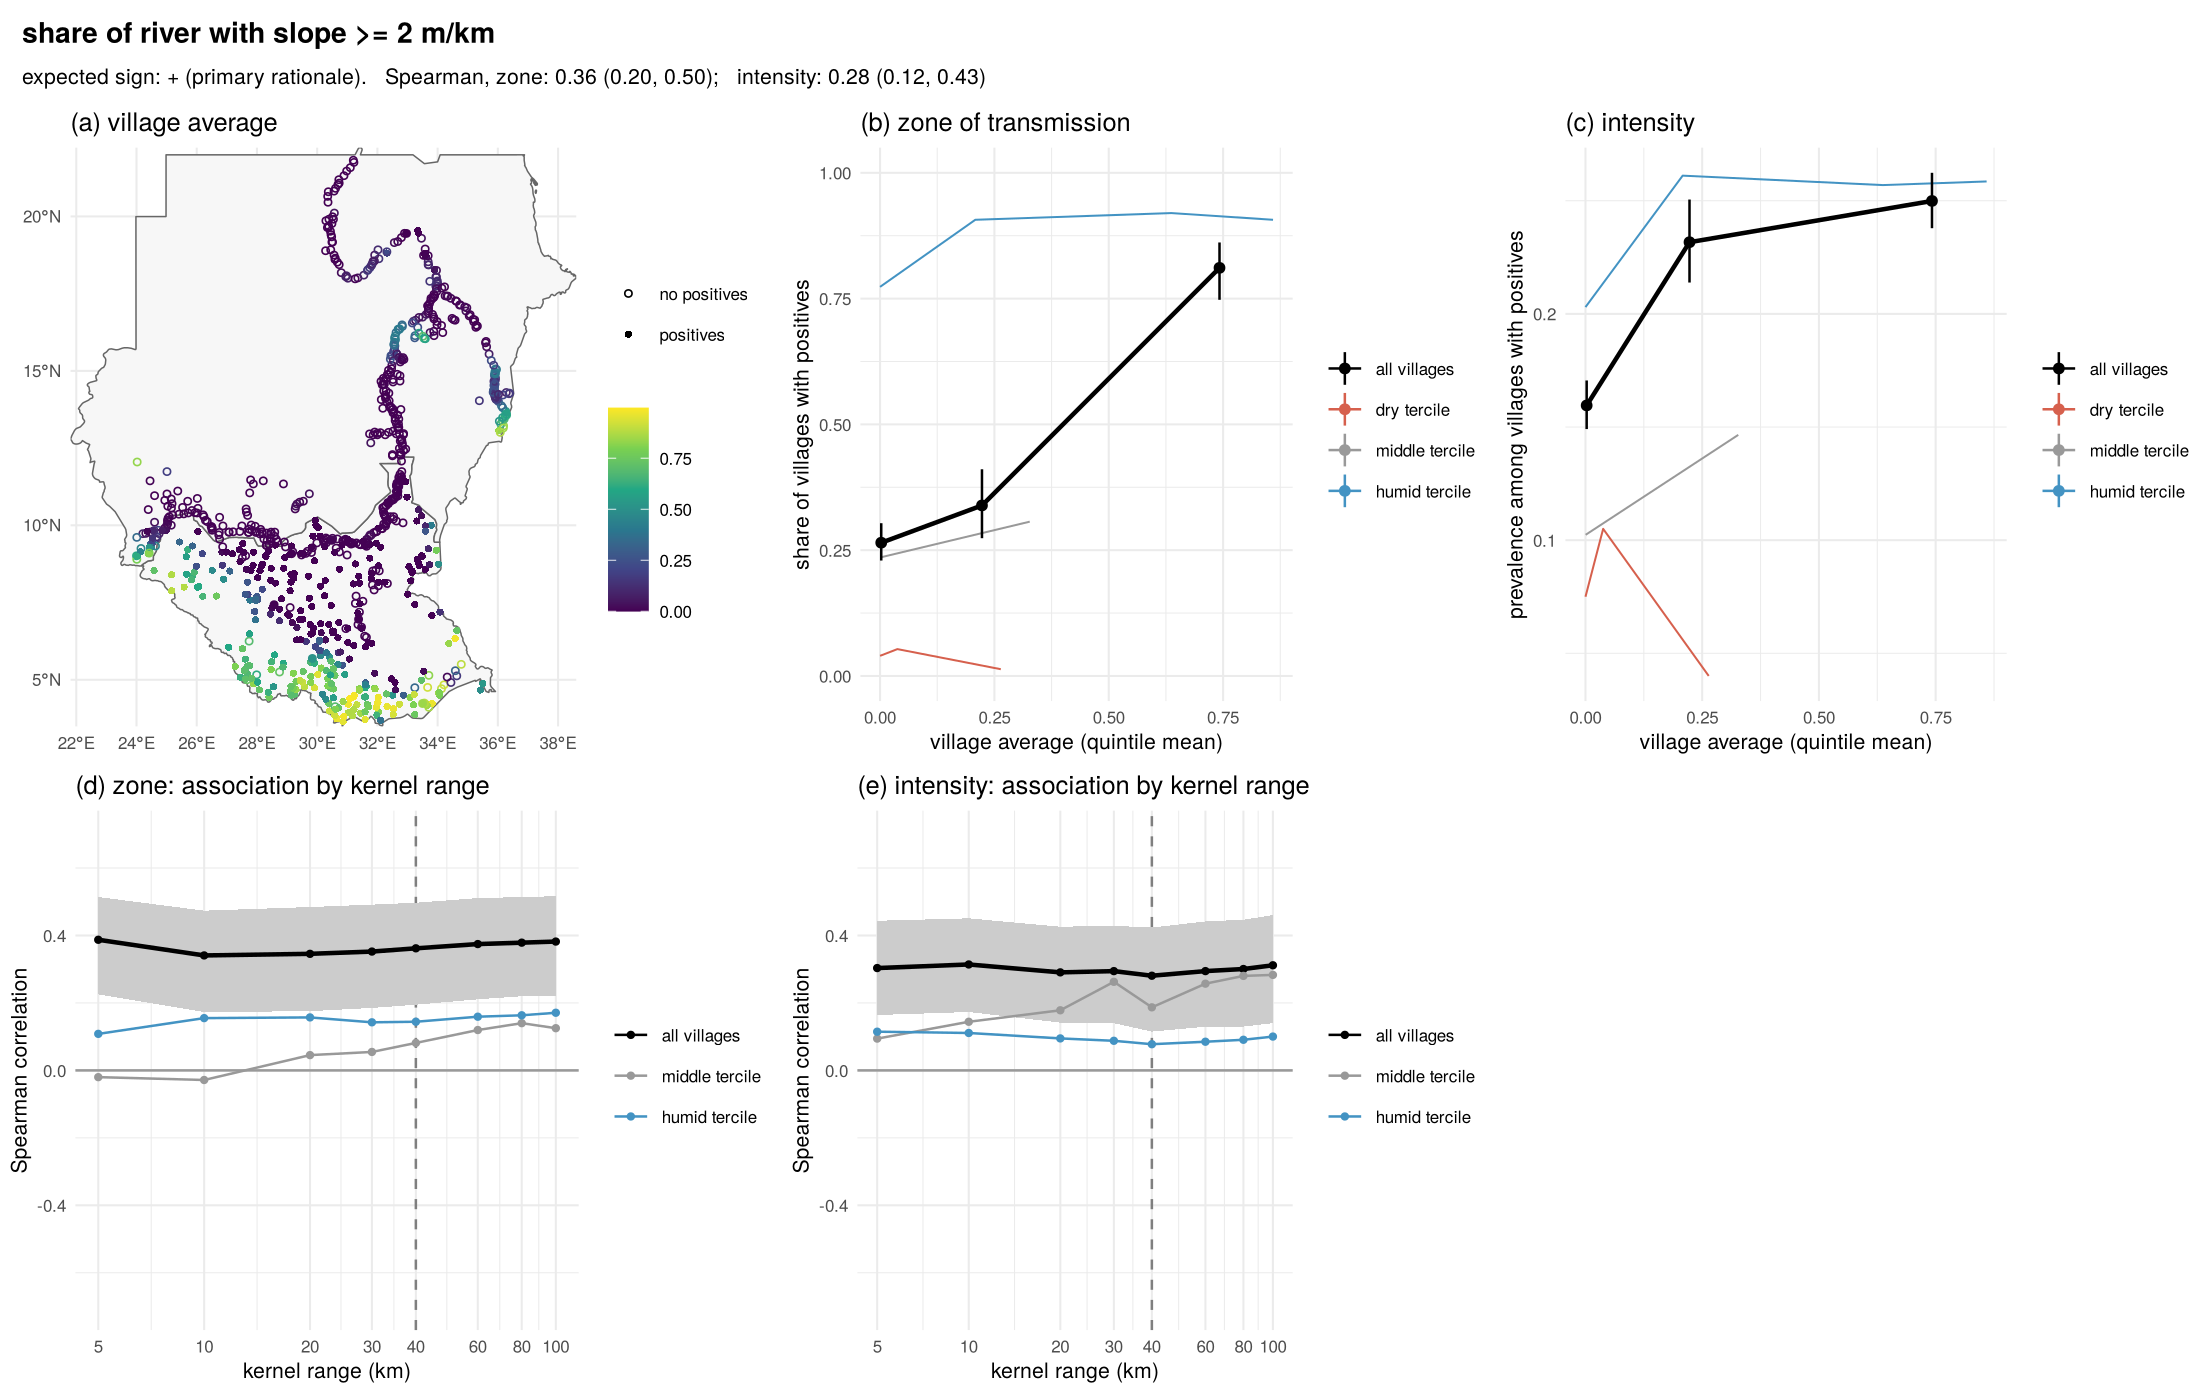
\includegraphics[width=\textwidth]{eda_steep_share.png}\caption{Share of river with slope of at least 2~m/km. Panels as in Figure~\ref{fig:slope}.}\label{fig:steep}\end{figure}
\begin{figure}[H]\centering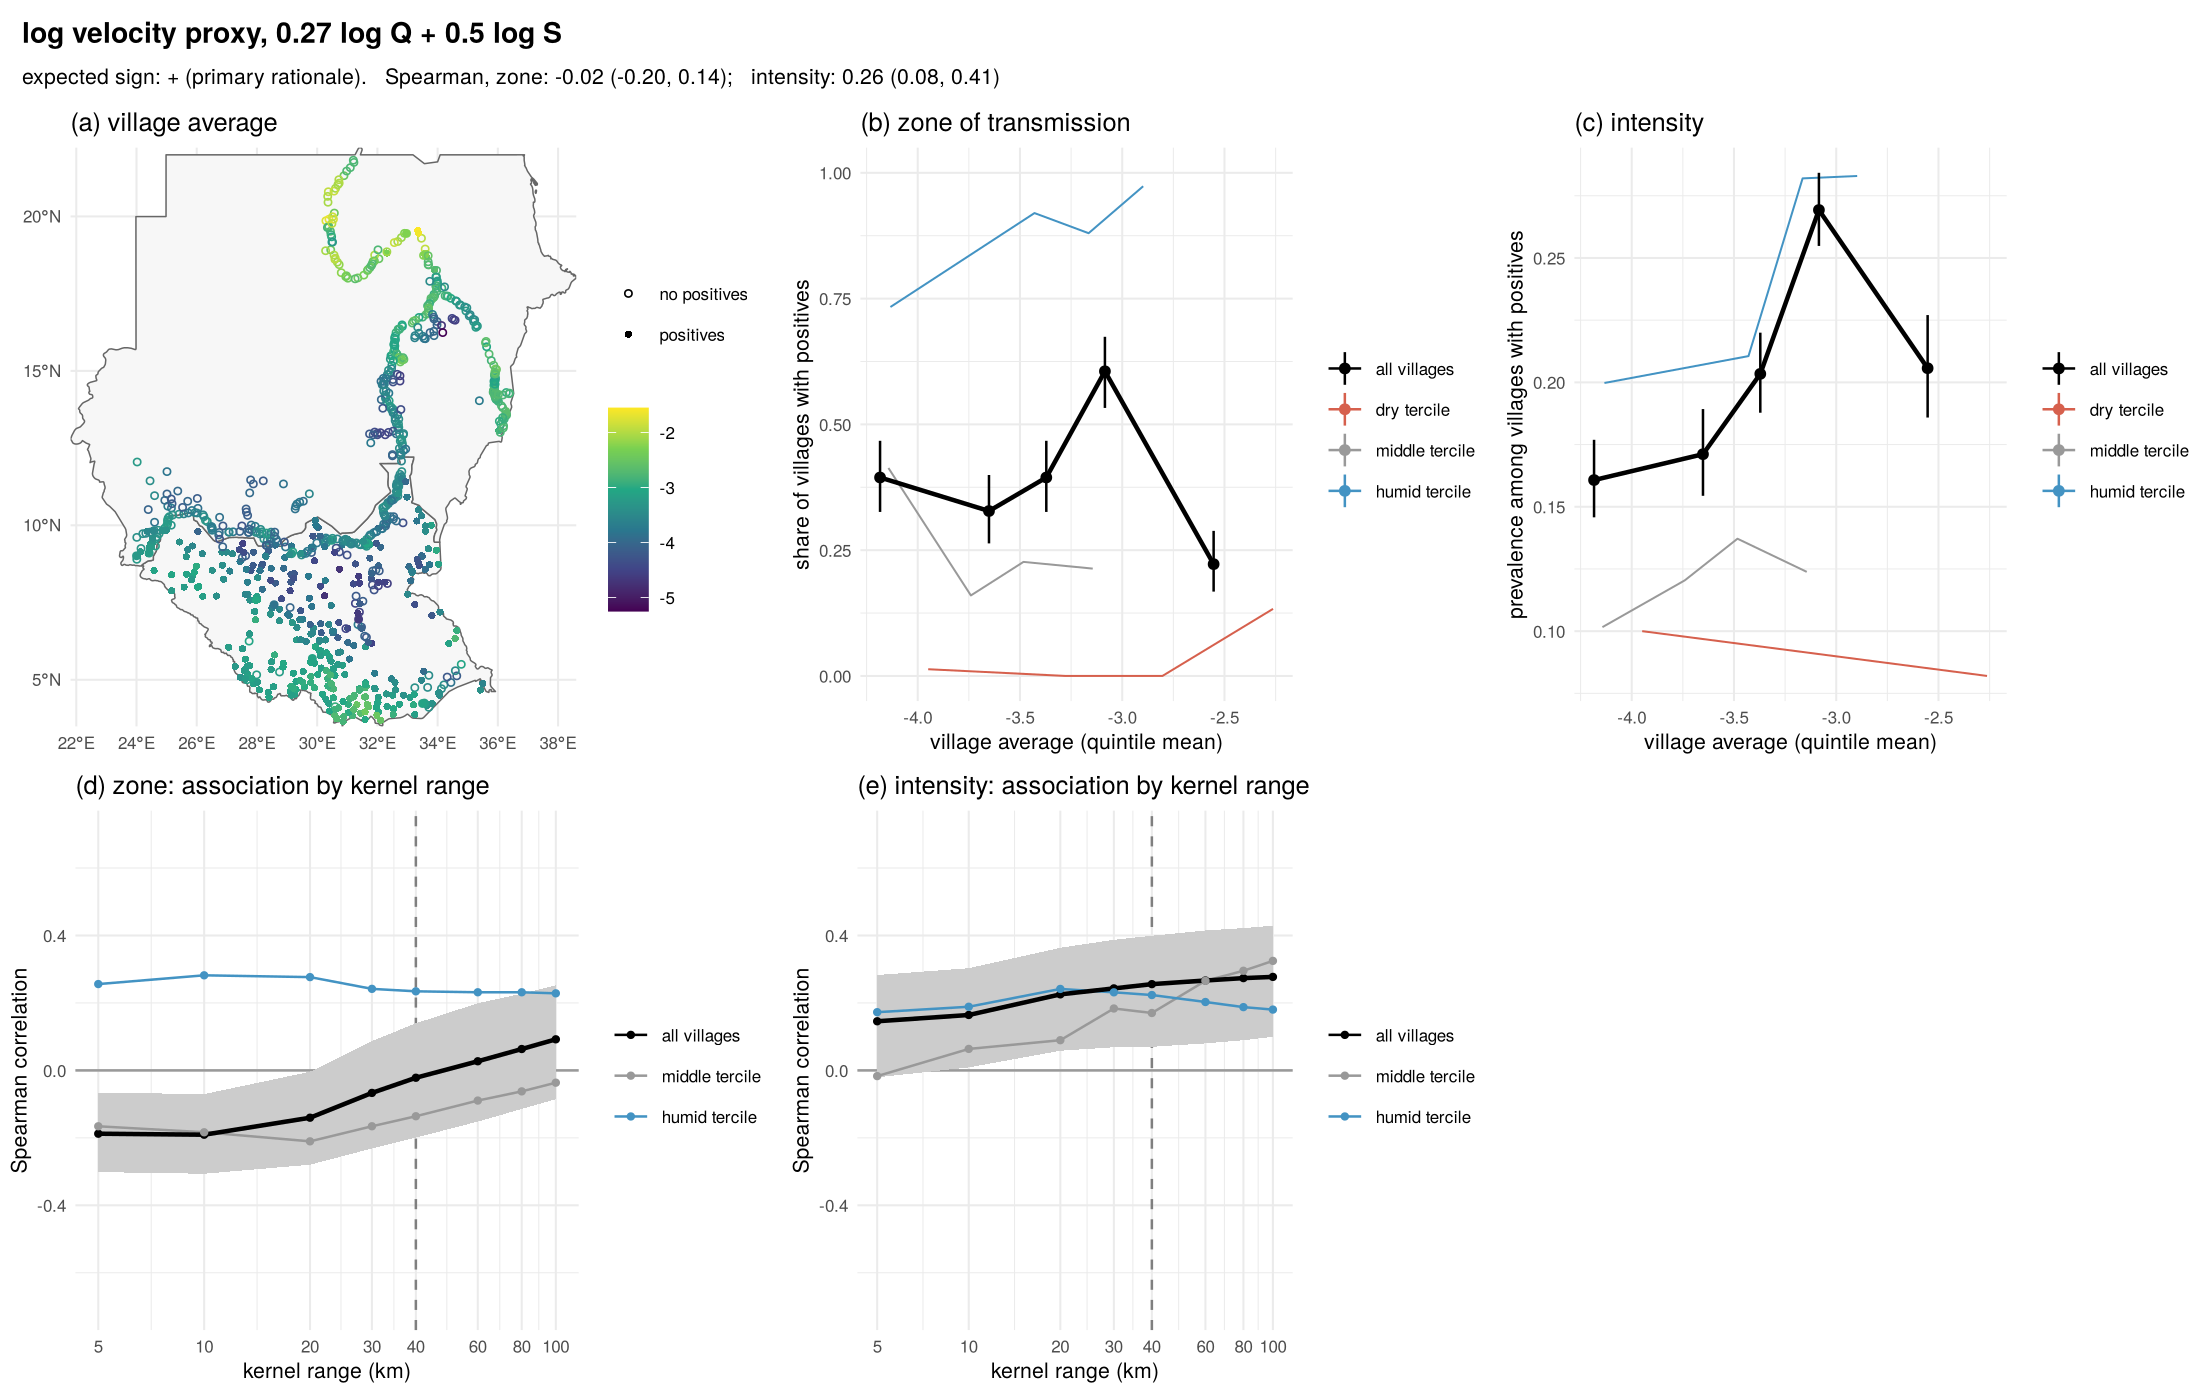
\includegraphics[width=\textwidth]{eda_velocity.png}\caption{Velocity proxy, $0.27\log Q + 0.5 \log S$. Panels as in Figure~\ref{fig:slope}.}\label{fig:velocity}\end{figure}
\begin{figure}[H]\centering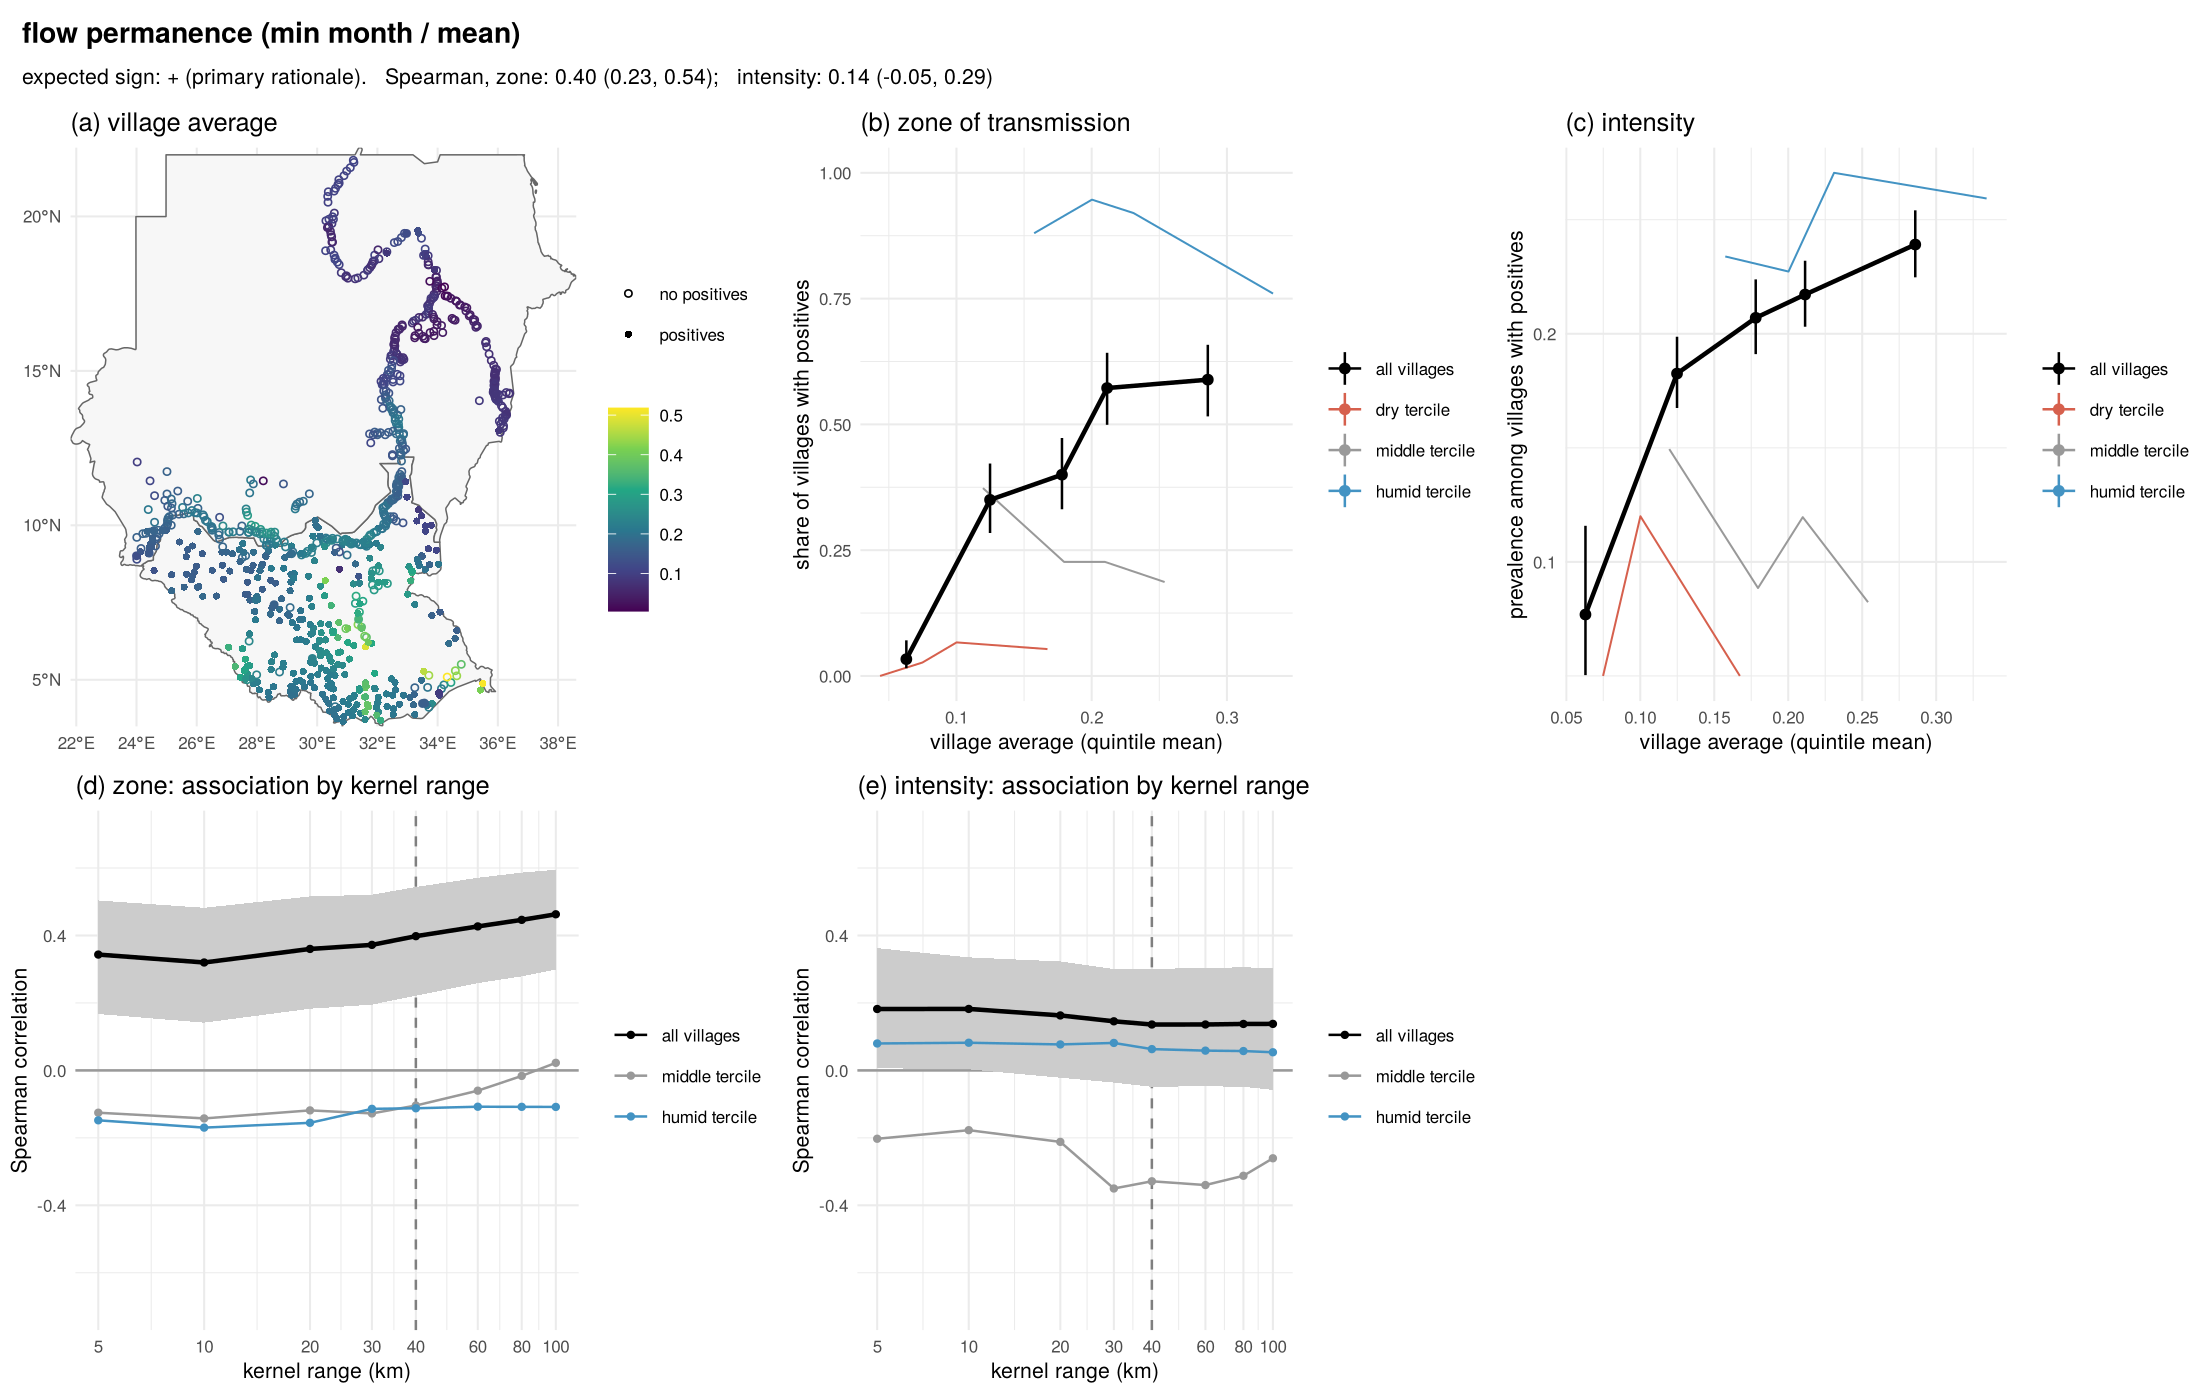
\includegraphics[width=\textwidth]{eda_permanence.png}\caption{Flow permanence, discharge of the driest month over the mean. Panels as in Figure~\ref{fig:slope}.}\label{fig:permanence}\end{figure}
\begin{figure}[H]\centering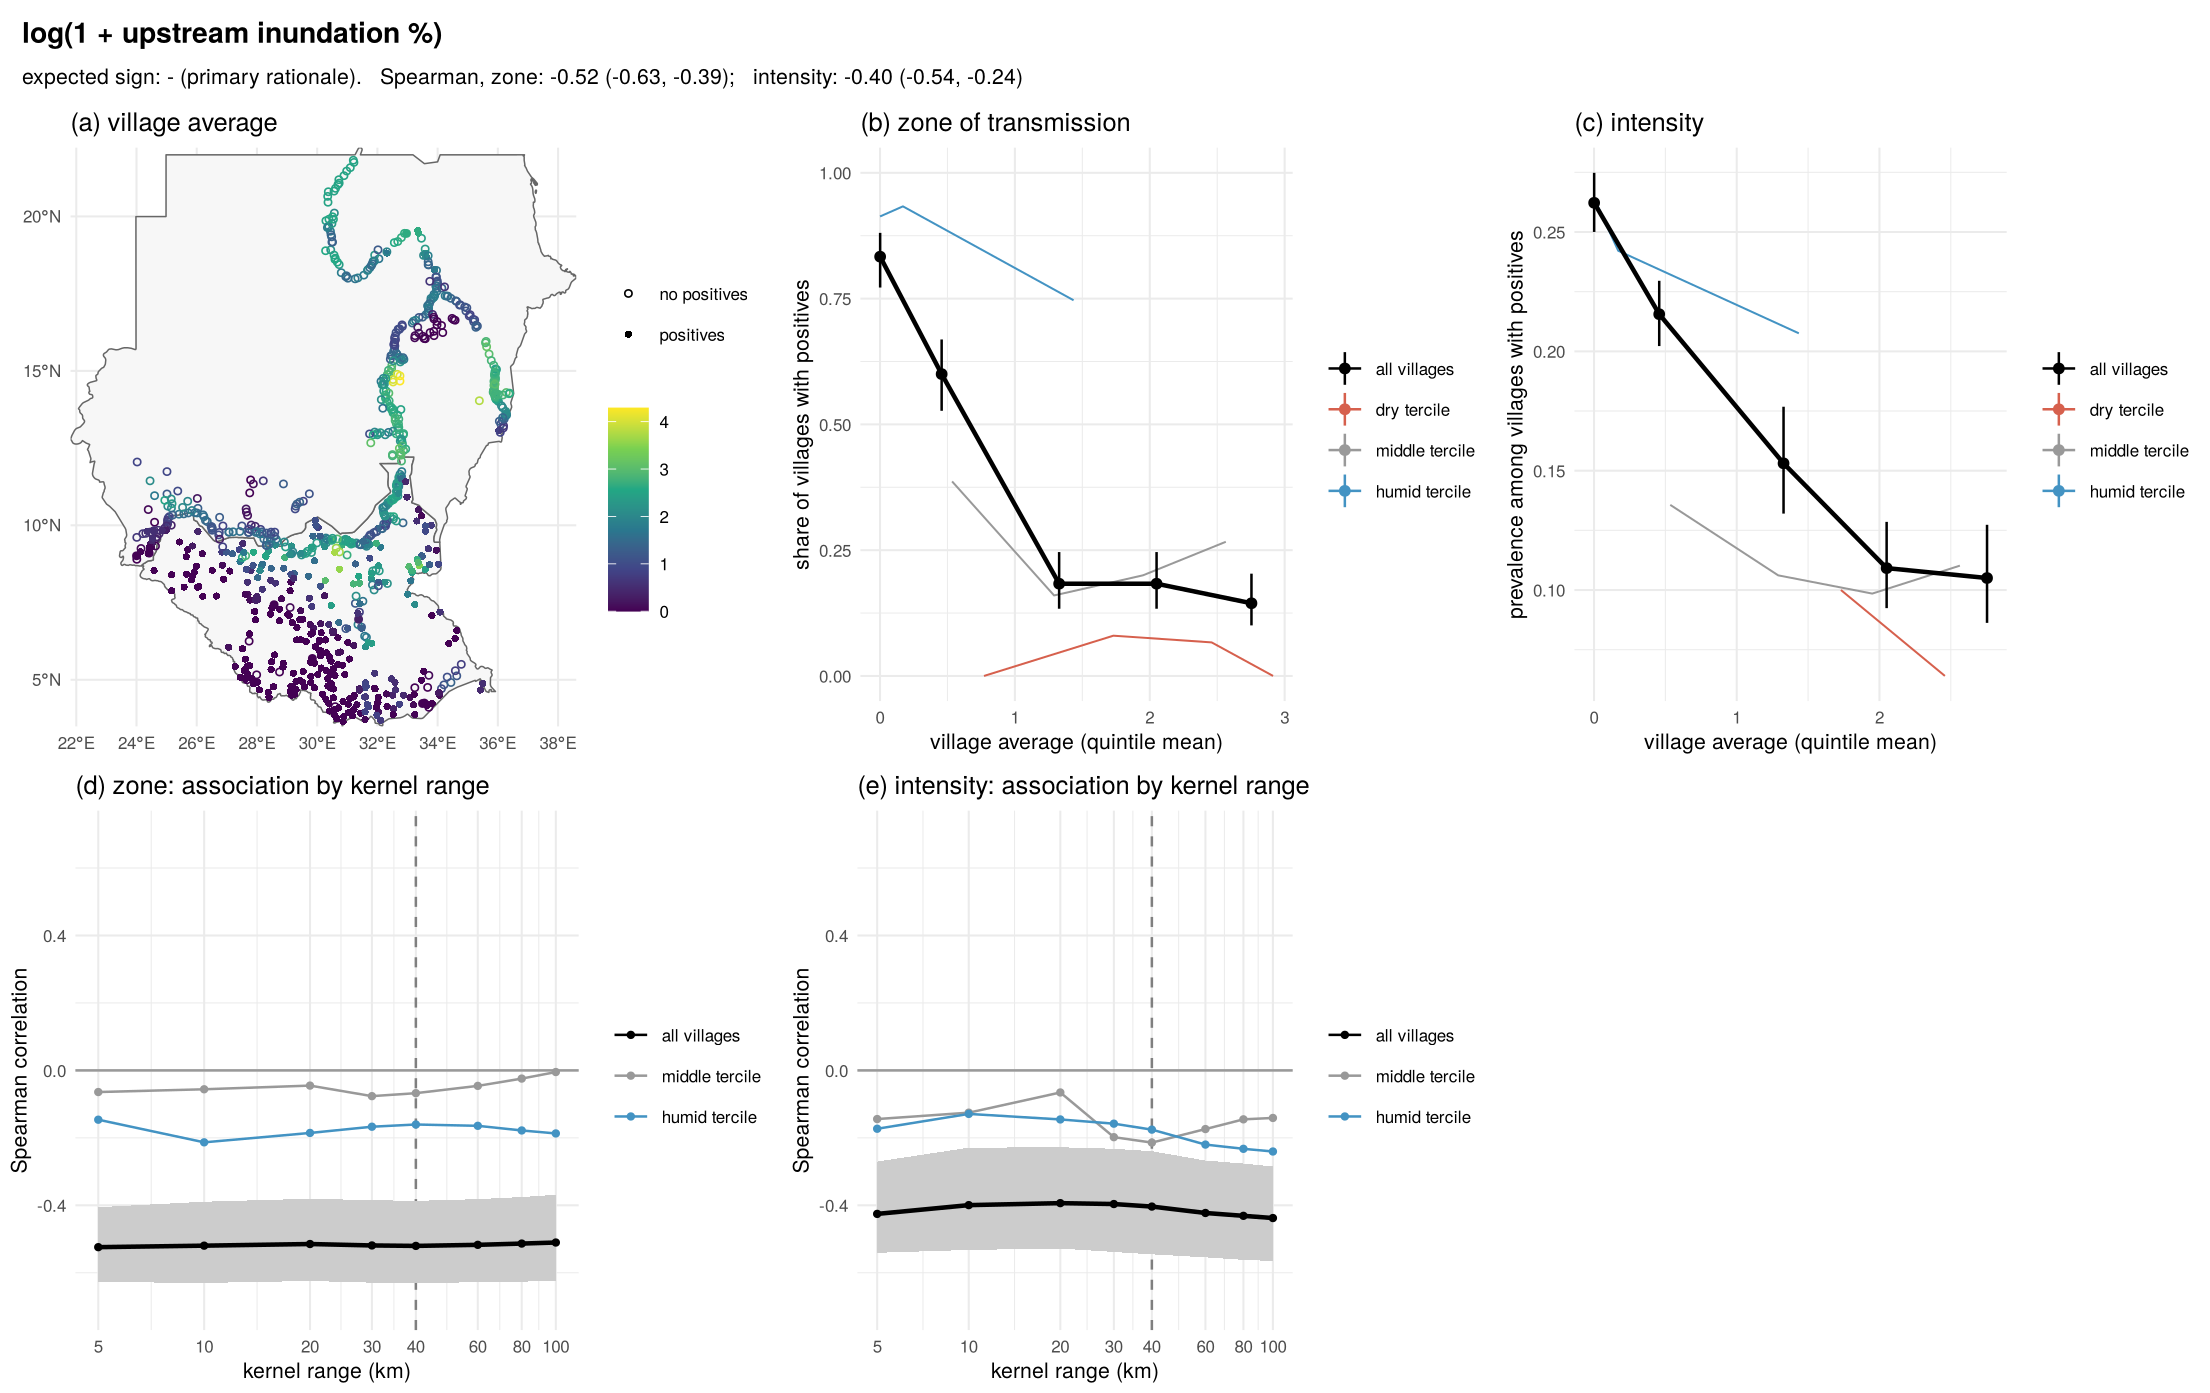
\includegraphics[width=\textwidth]{eda_inundation.png}\caption{Upstream inundation extent. Panels as in Figure~\ref{fig:slope}.}\label{fig:inundation}\end{figure}
\begin{figure}[H]\centering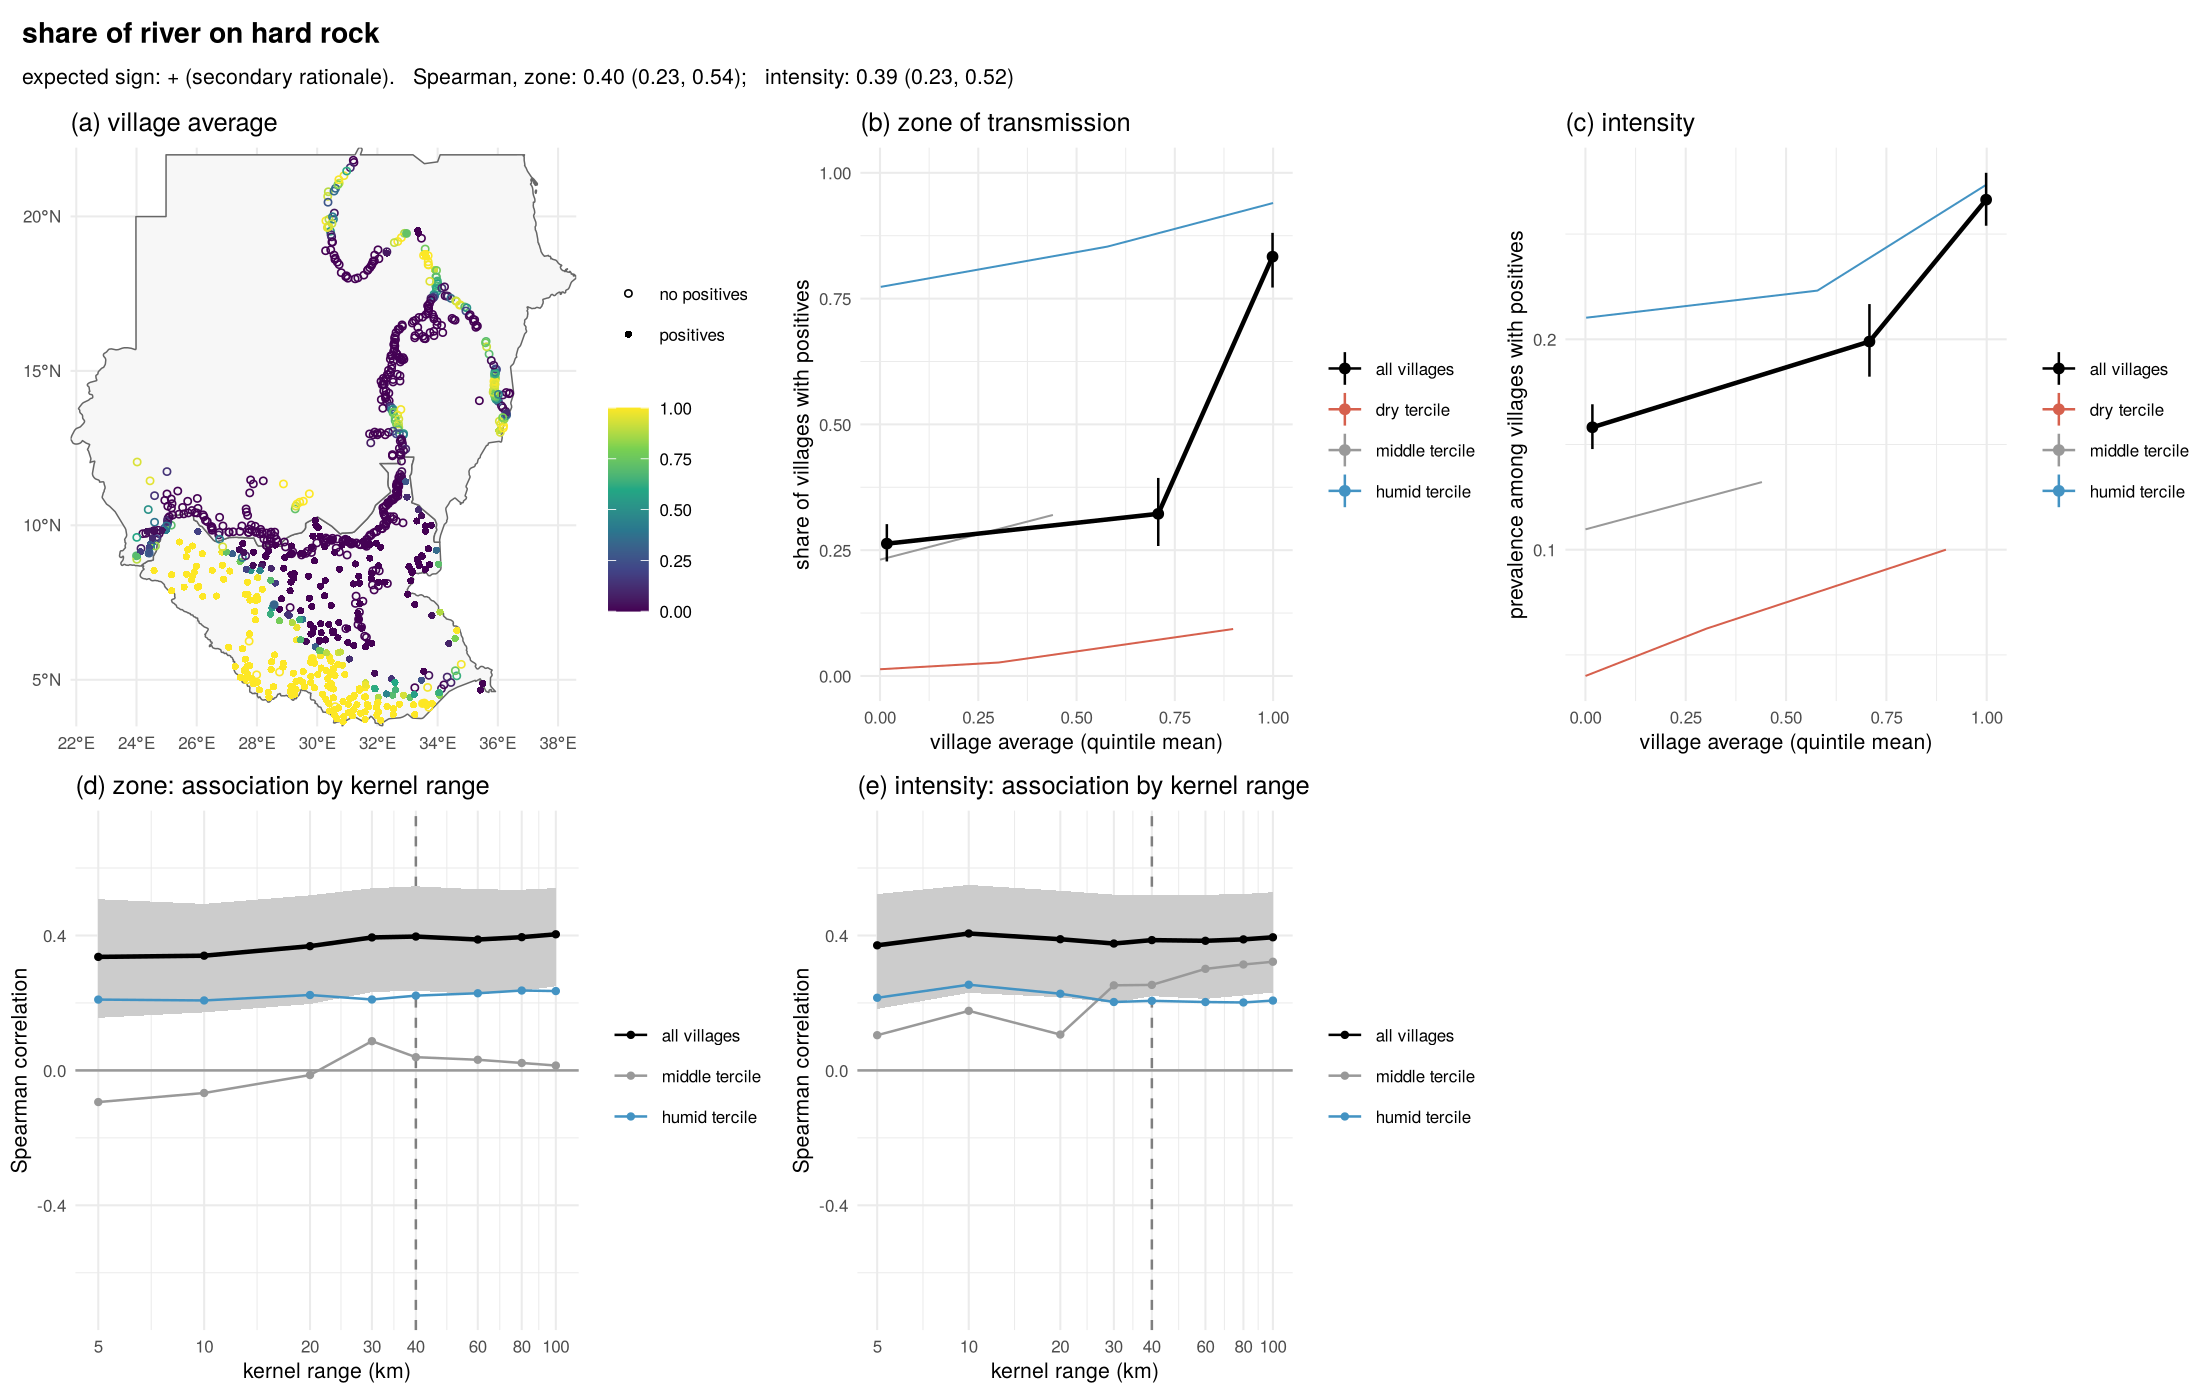
\includegraphics[width=\textwidth]{eda_hard_rock.png}\caption{Share of river on hard rock (basement and volcanic rocks). Panels as in Figure~\ref{fig:slope}.}\label{fig:hardrock}\end{figure}
\begin{figure}[H]\centering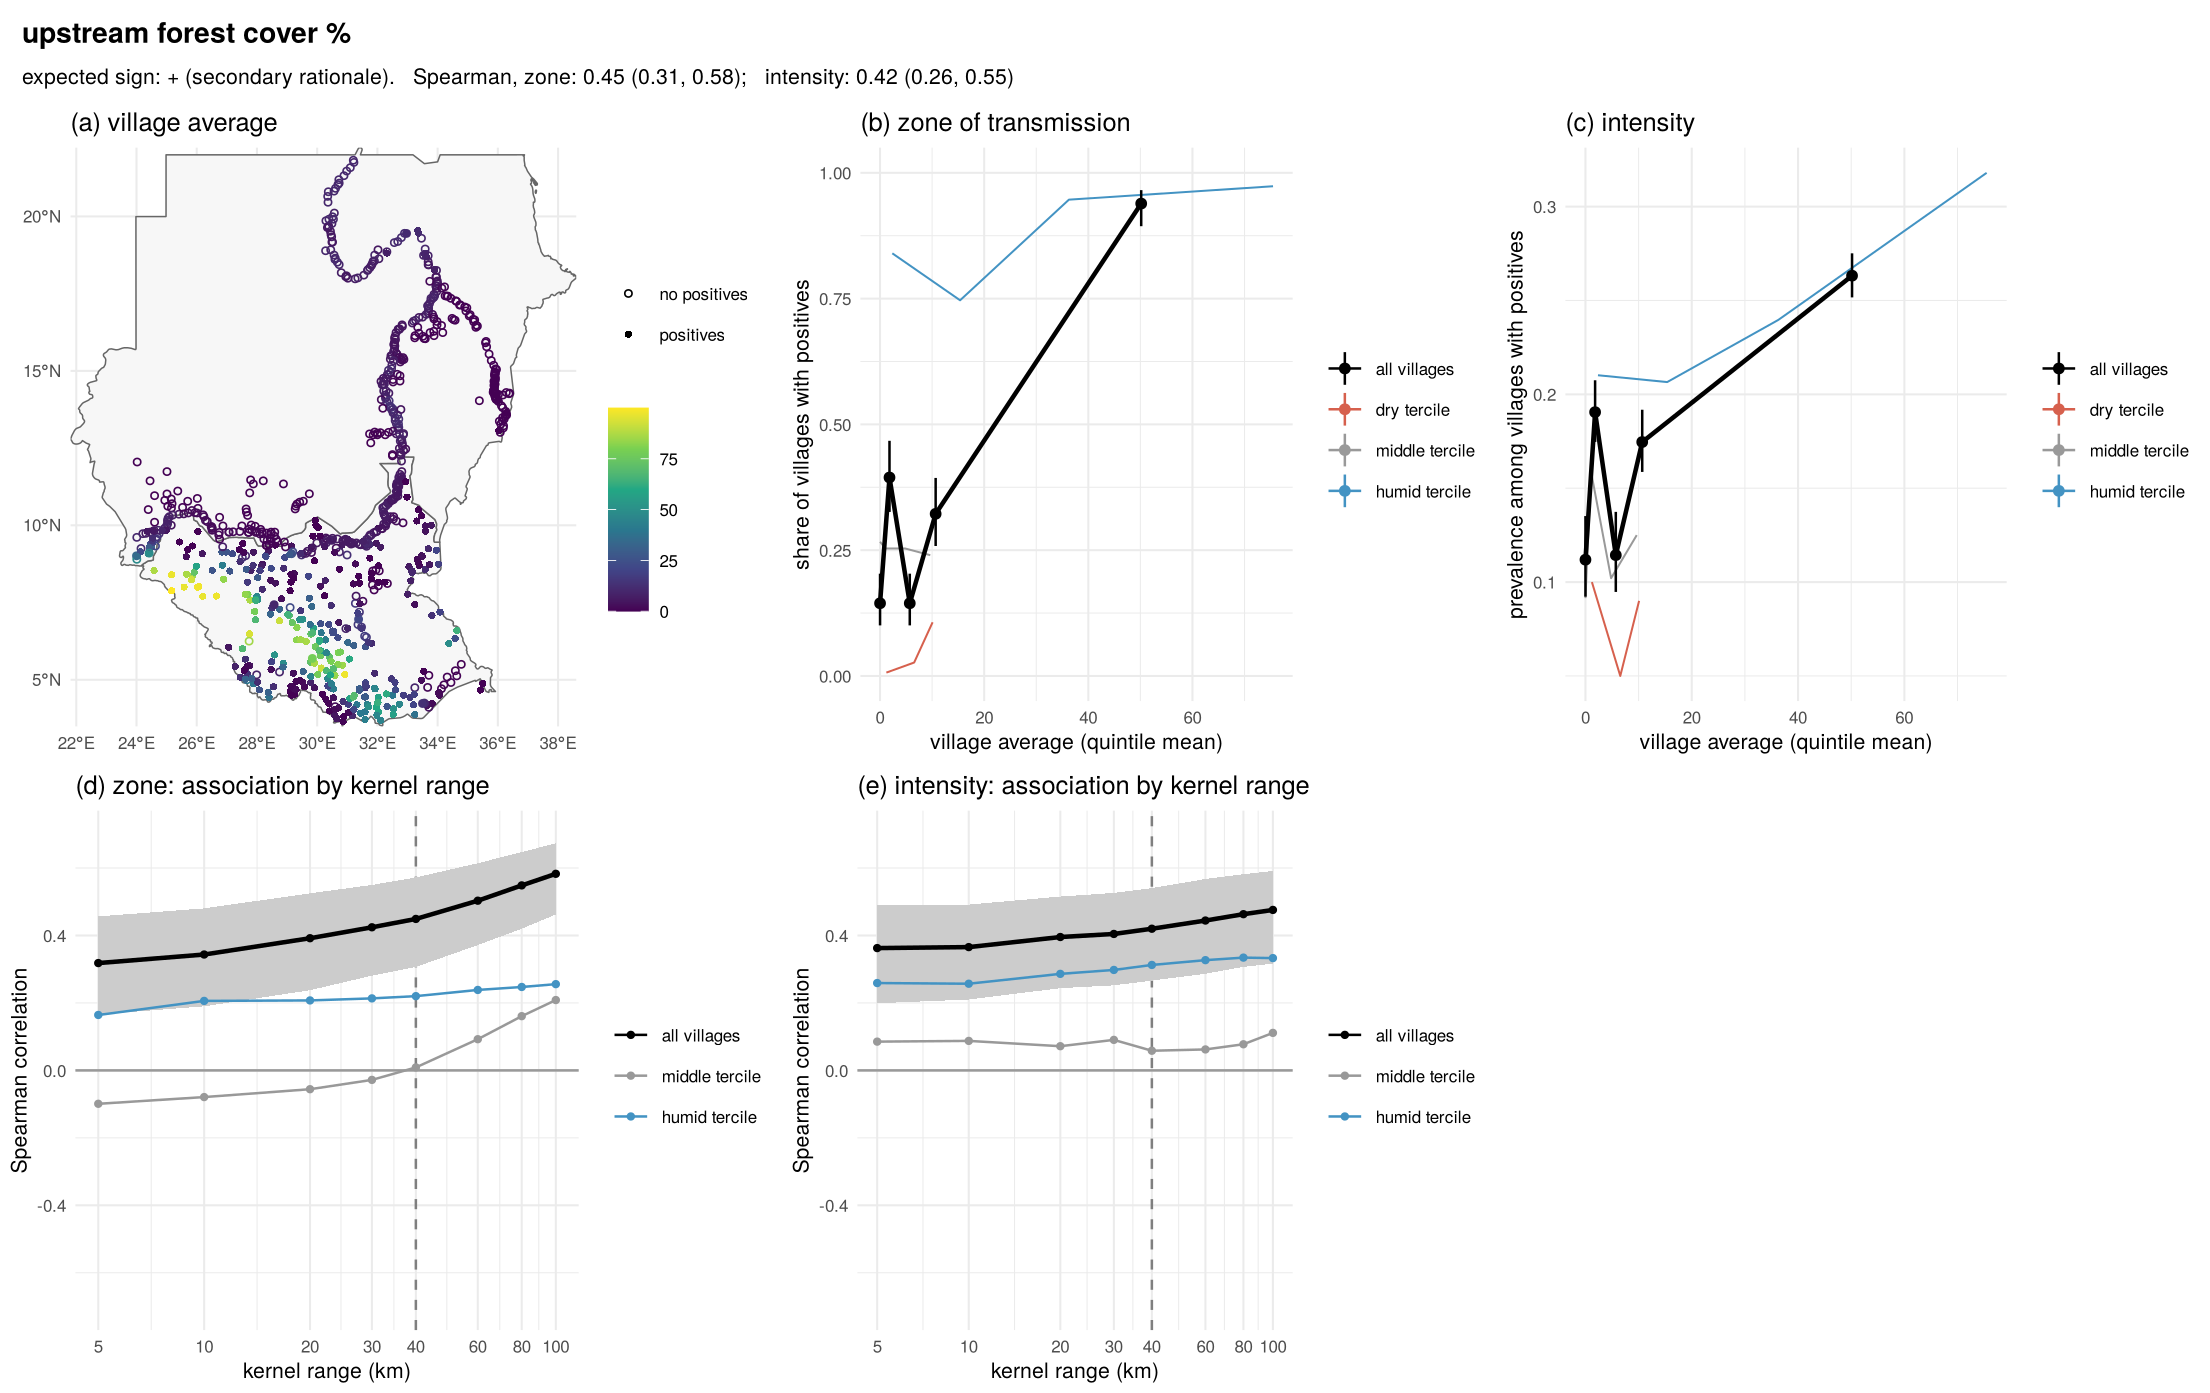
\includegraphics[width=\textwidth]{eda_forest.png}\caption{Upstream forest cover. Panels as in Figure~\ref{fig:slope}.}\label{fig:forest}\end{figure}
\begin{figure}[H]\centering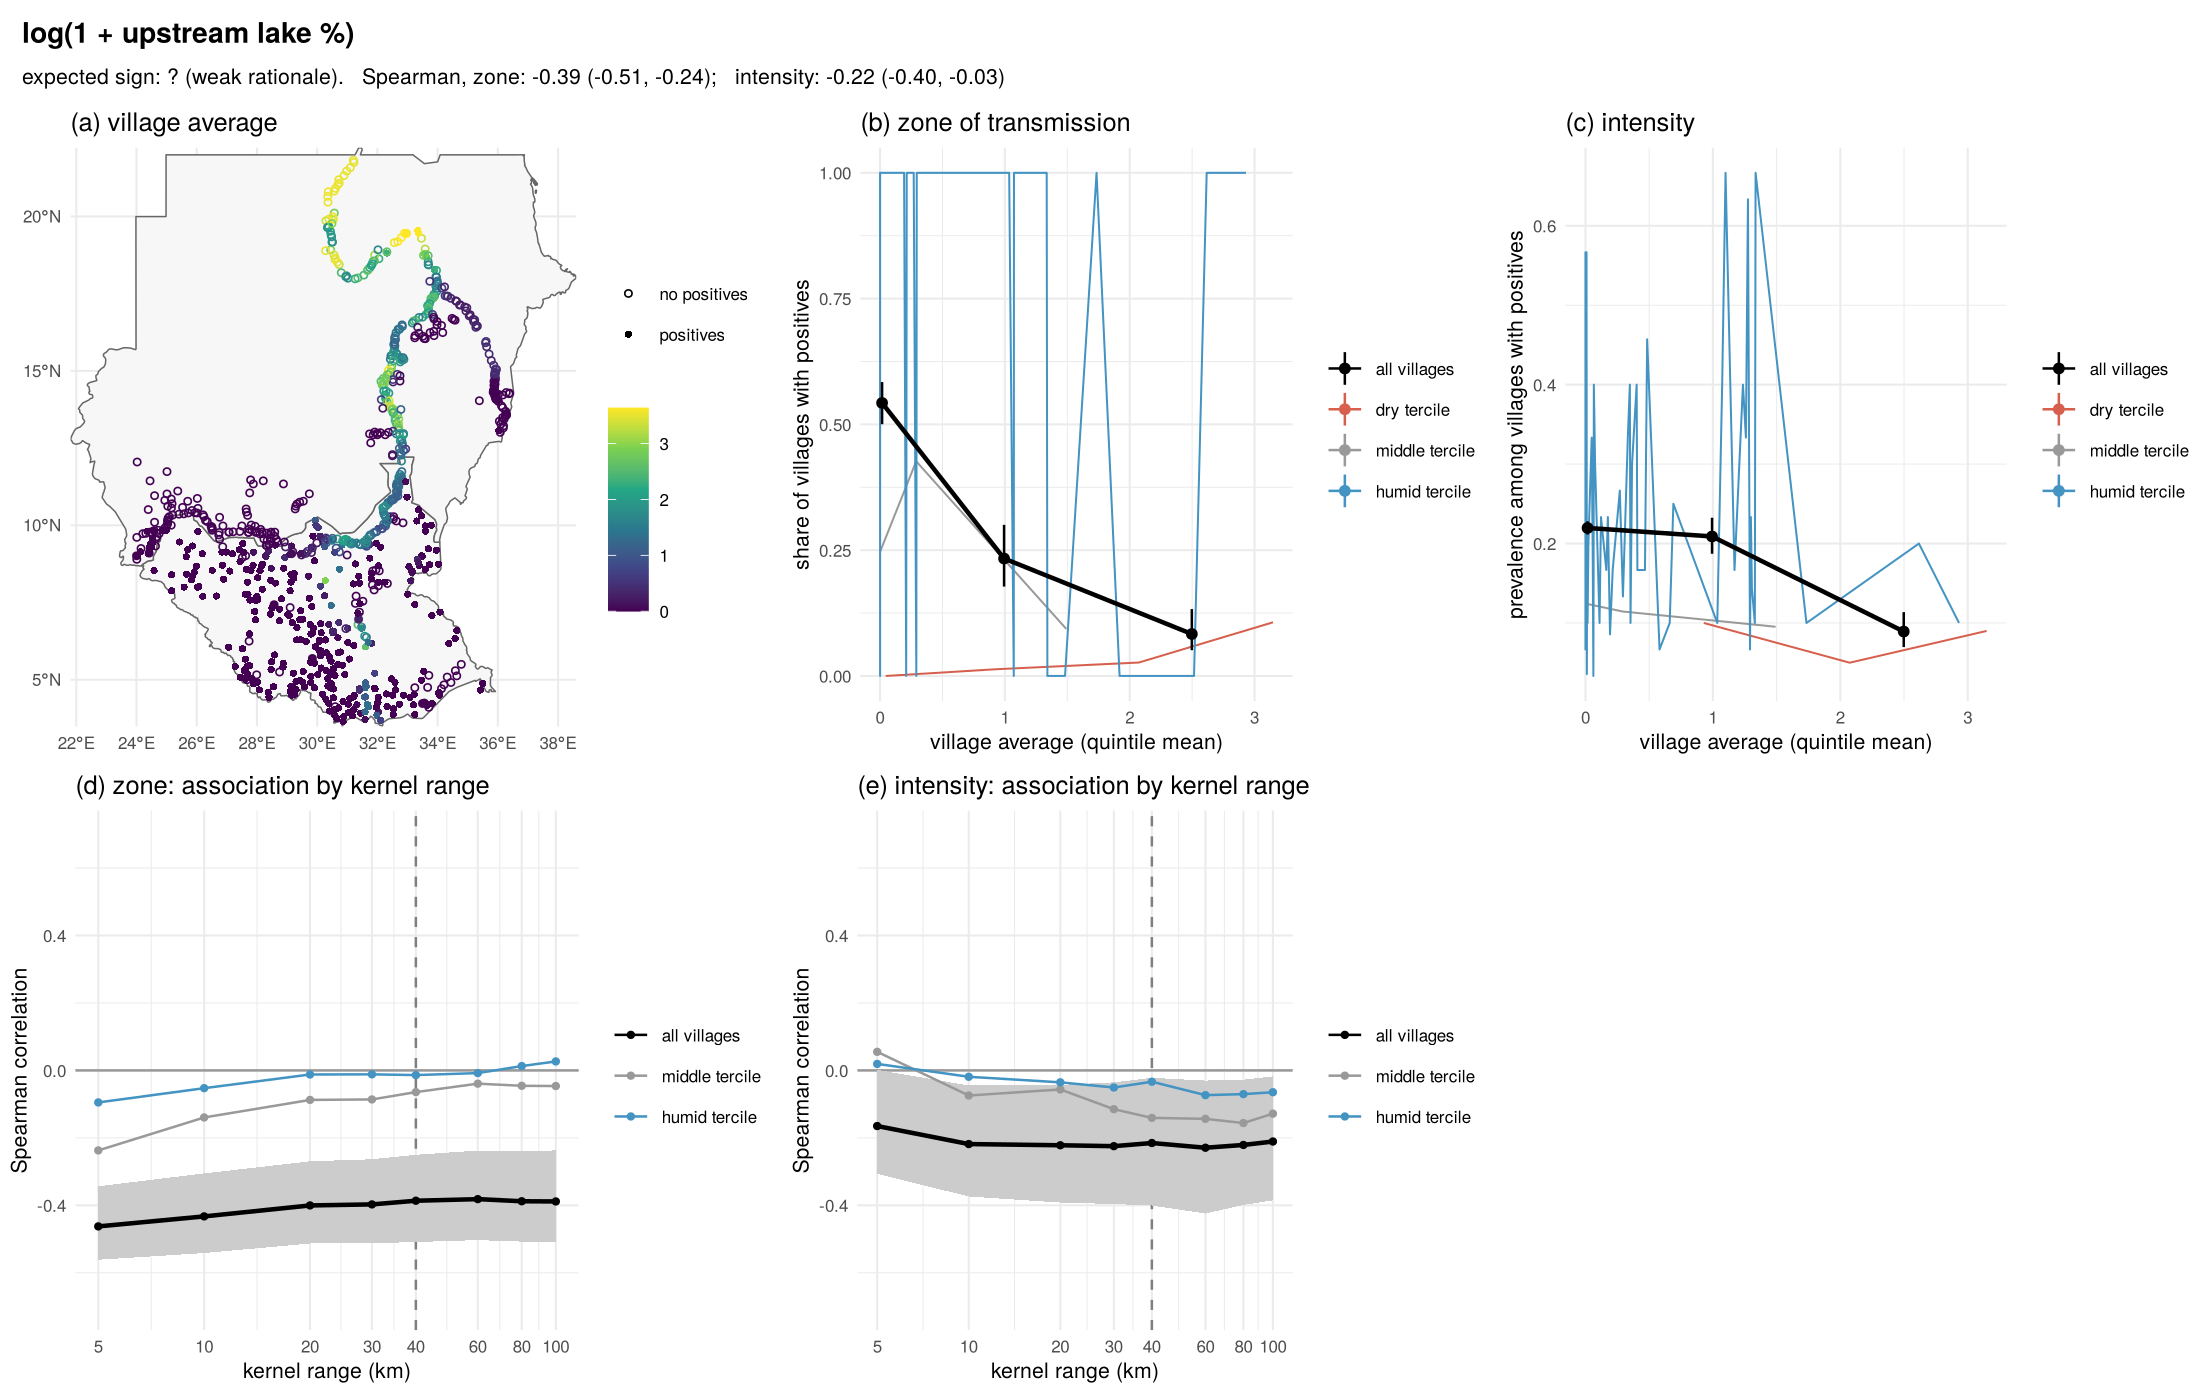
\includegraphics[width=\textwidth]{eda_lakes.png}\caption{Upstream lake area. Panels as in Figure~\ref{fig:slope}.}\label{fig:lakes}\end{figure}
\begin{figure}[H]\centering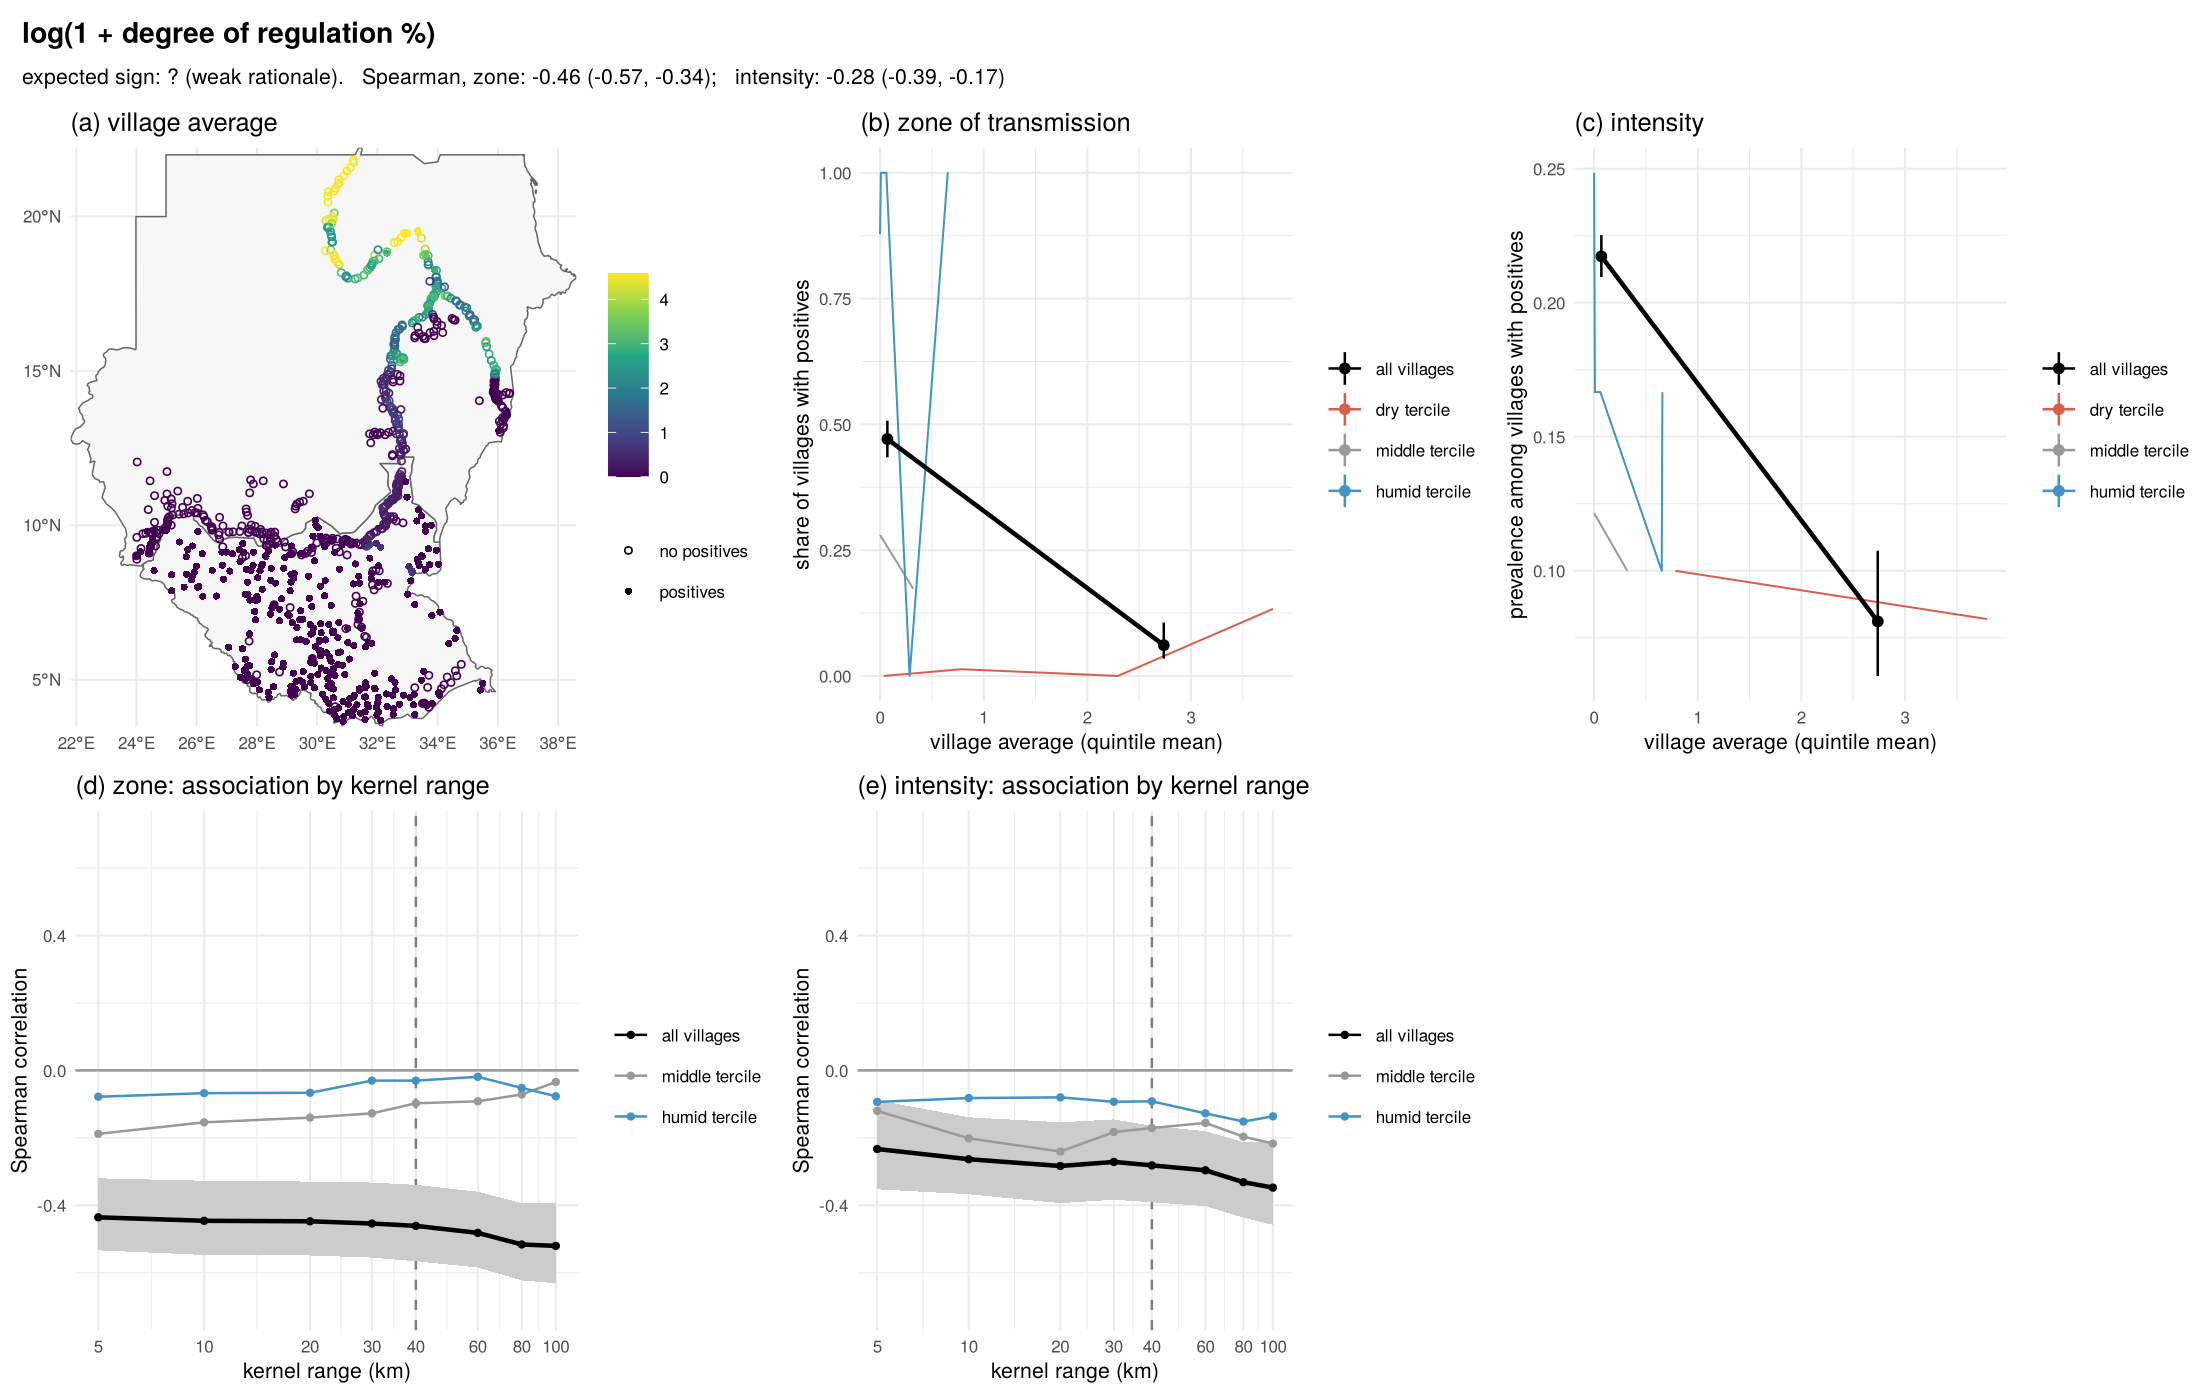
\includegraphics[width=\textwidth]{eda_regulation.png}\caption{Degree of regulation by dams. Panels as in Figure~\ref{fig:slope}.}\label{fig:regulation}\end{figure}
\begin{figure}[H]\centering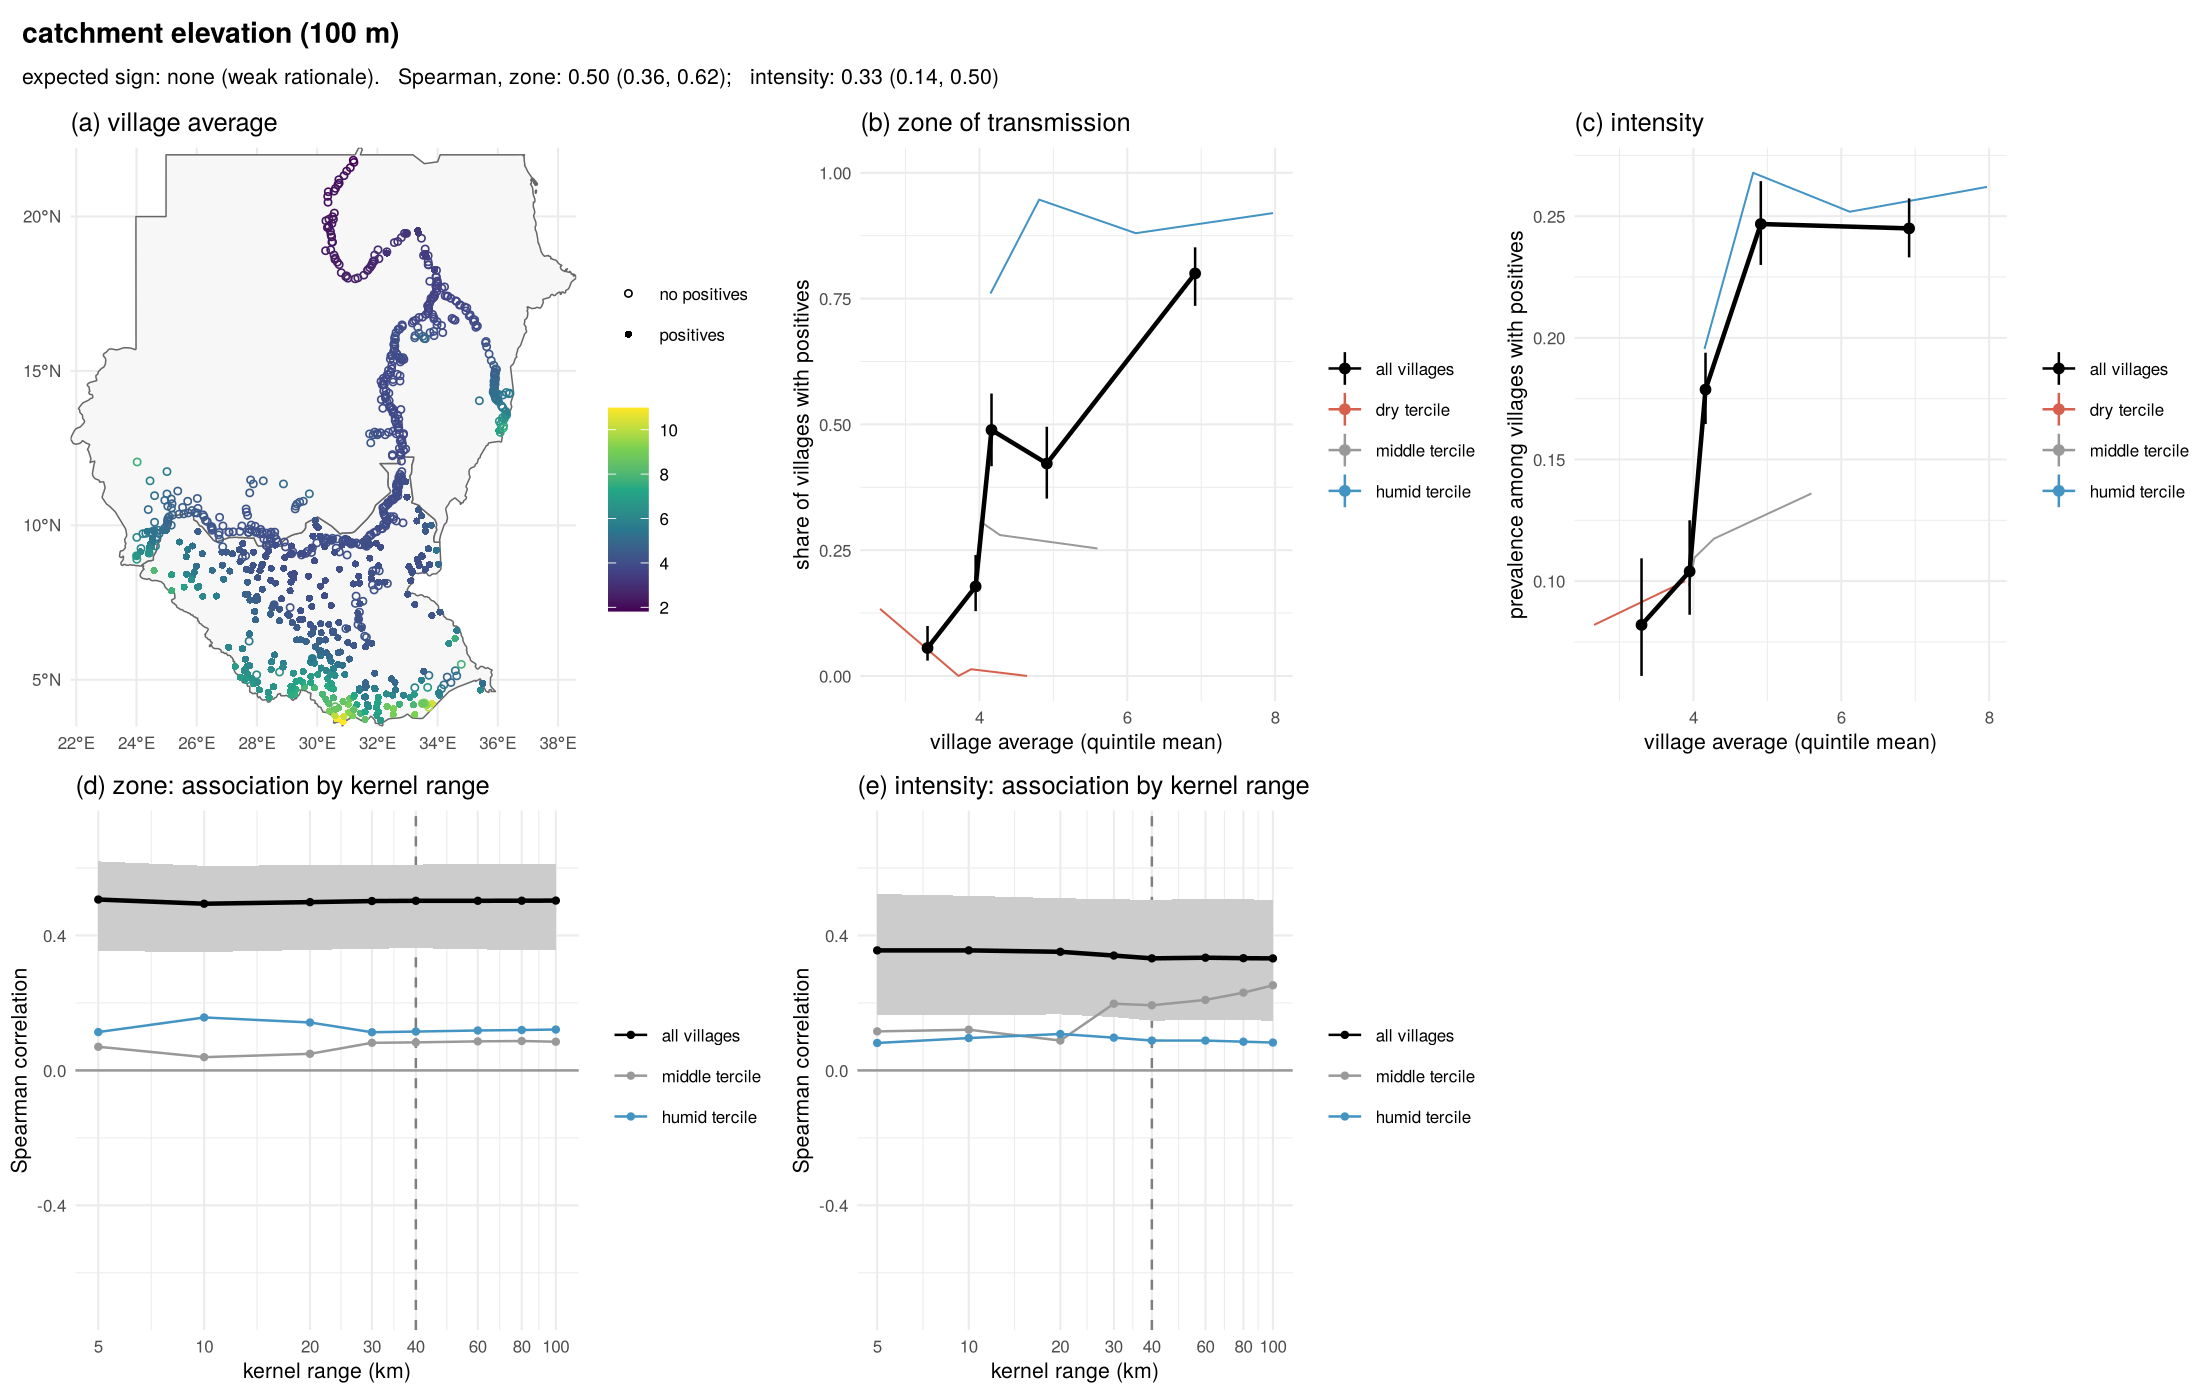
\includegraphics[width=\textwidth]{eda_elevation.png}\caption{Catchment elevation. Panels as in Figure~\ref{fig:slope}.}\label{fig:elevation}\end{figure}
\begin{figure}[H]\centering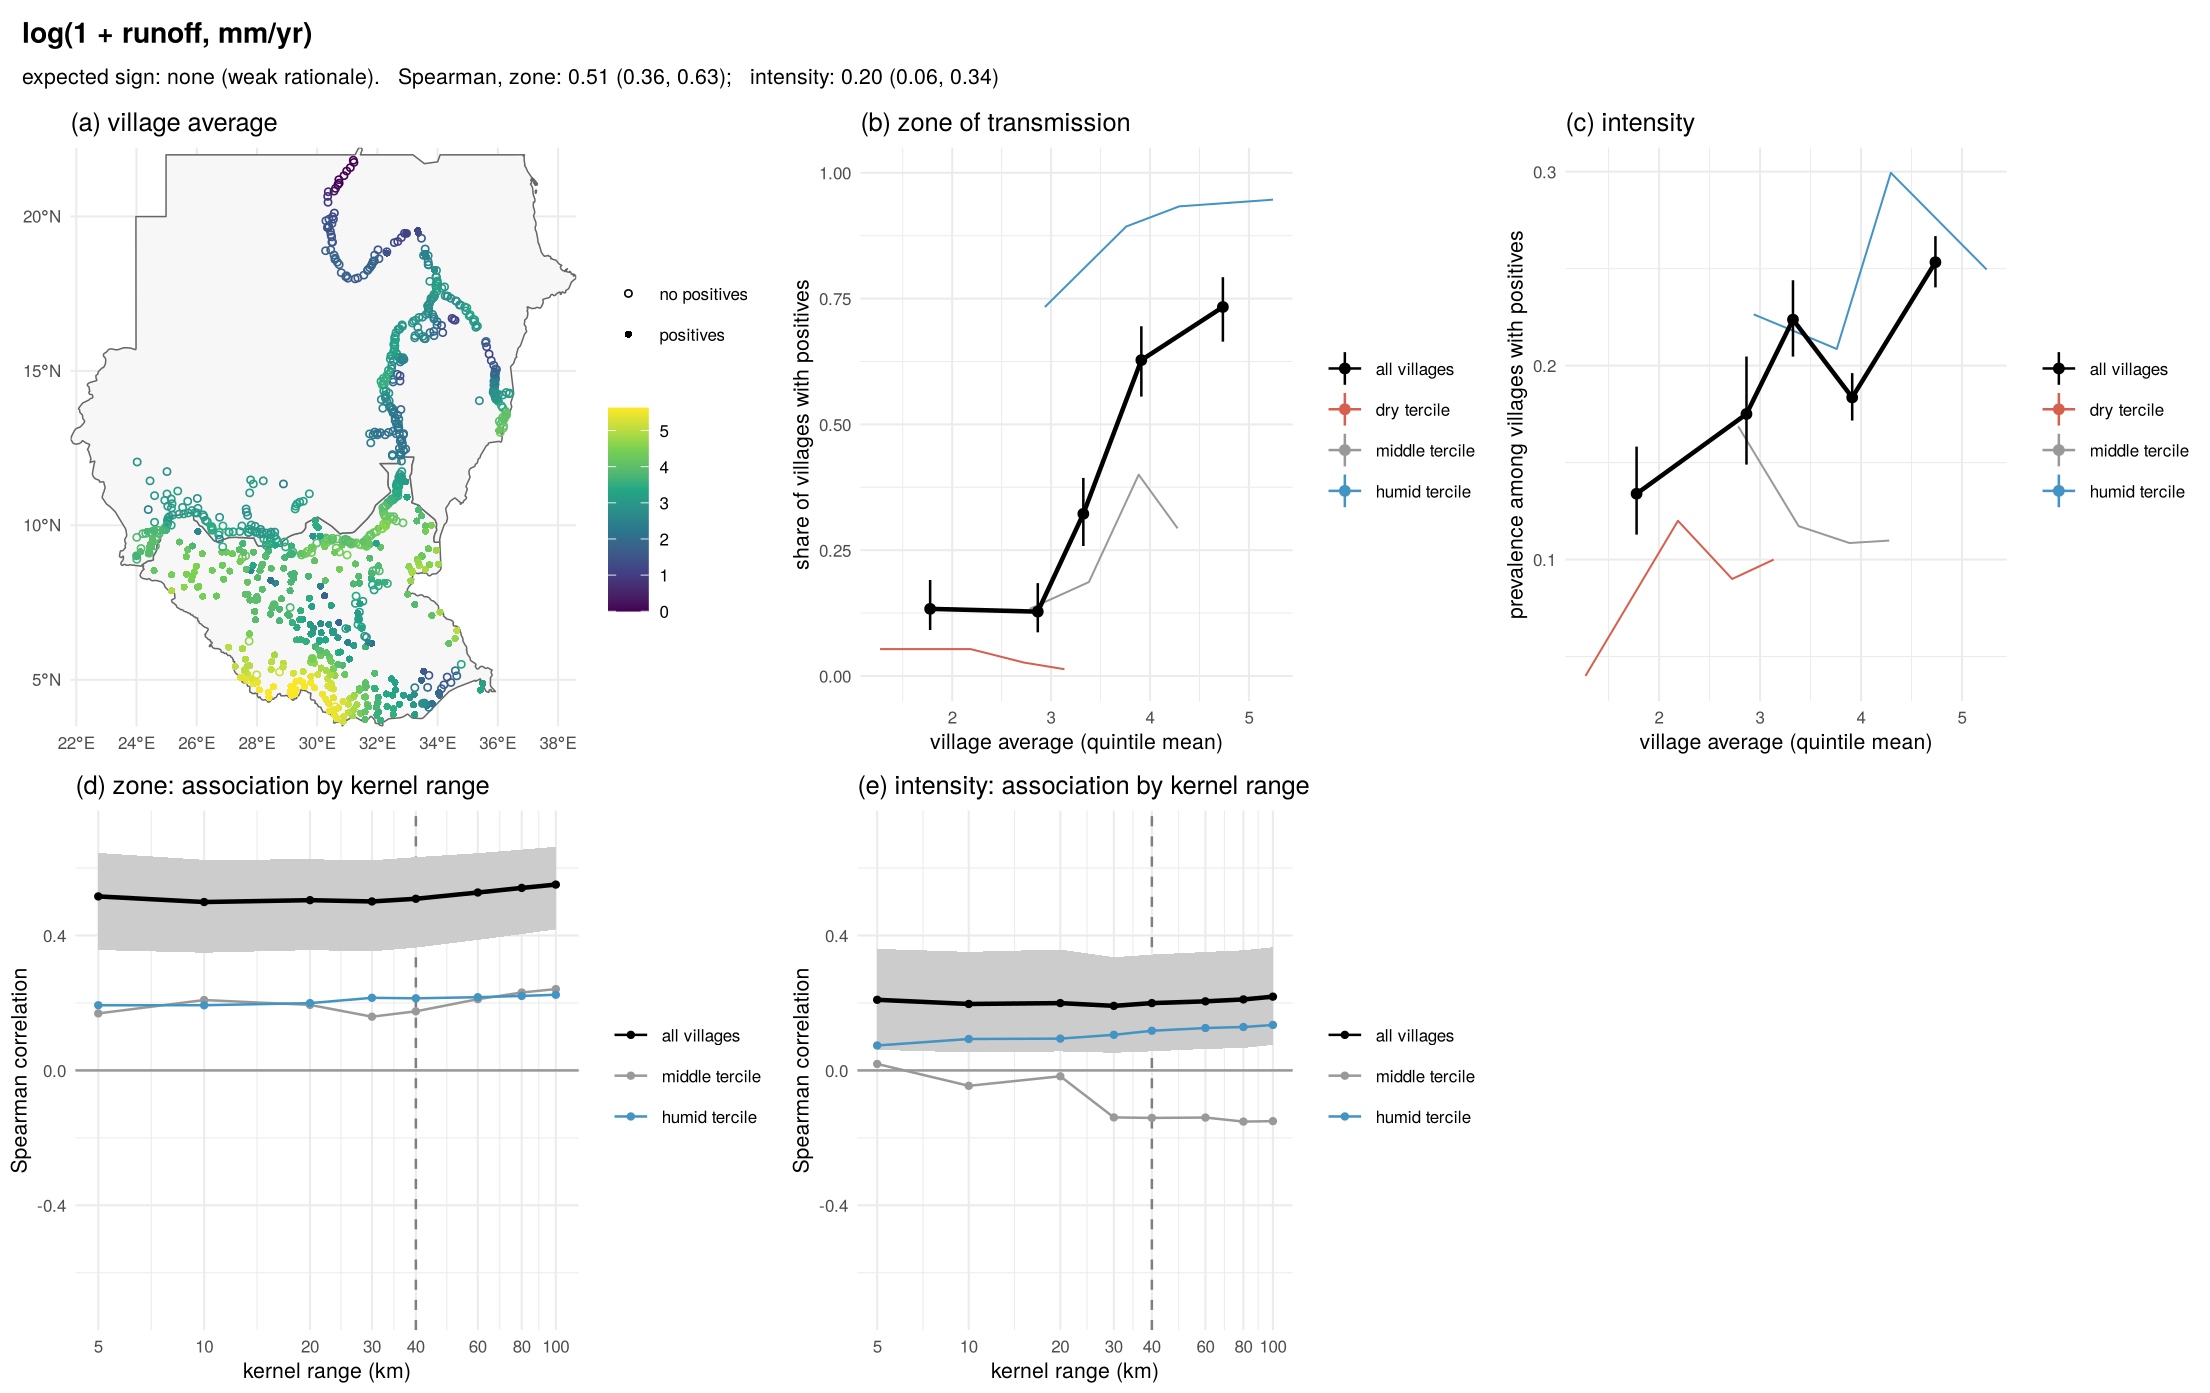
\includegraphics[width=\textwidth]{eda_runoff.png}\caption{Runoff. Panels as in Figure~\ref{fig:slope}.}\label{fig:runoff}\end{figure}
\begin{figure}[H]\centering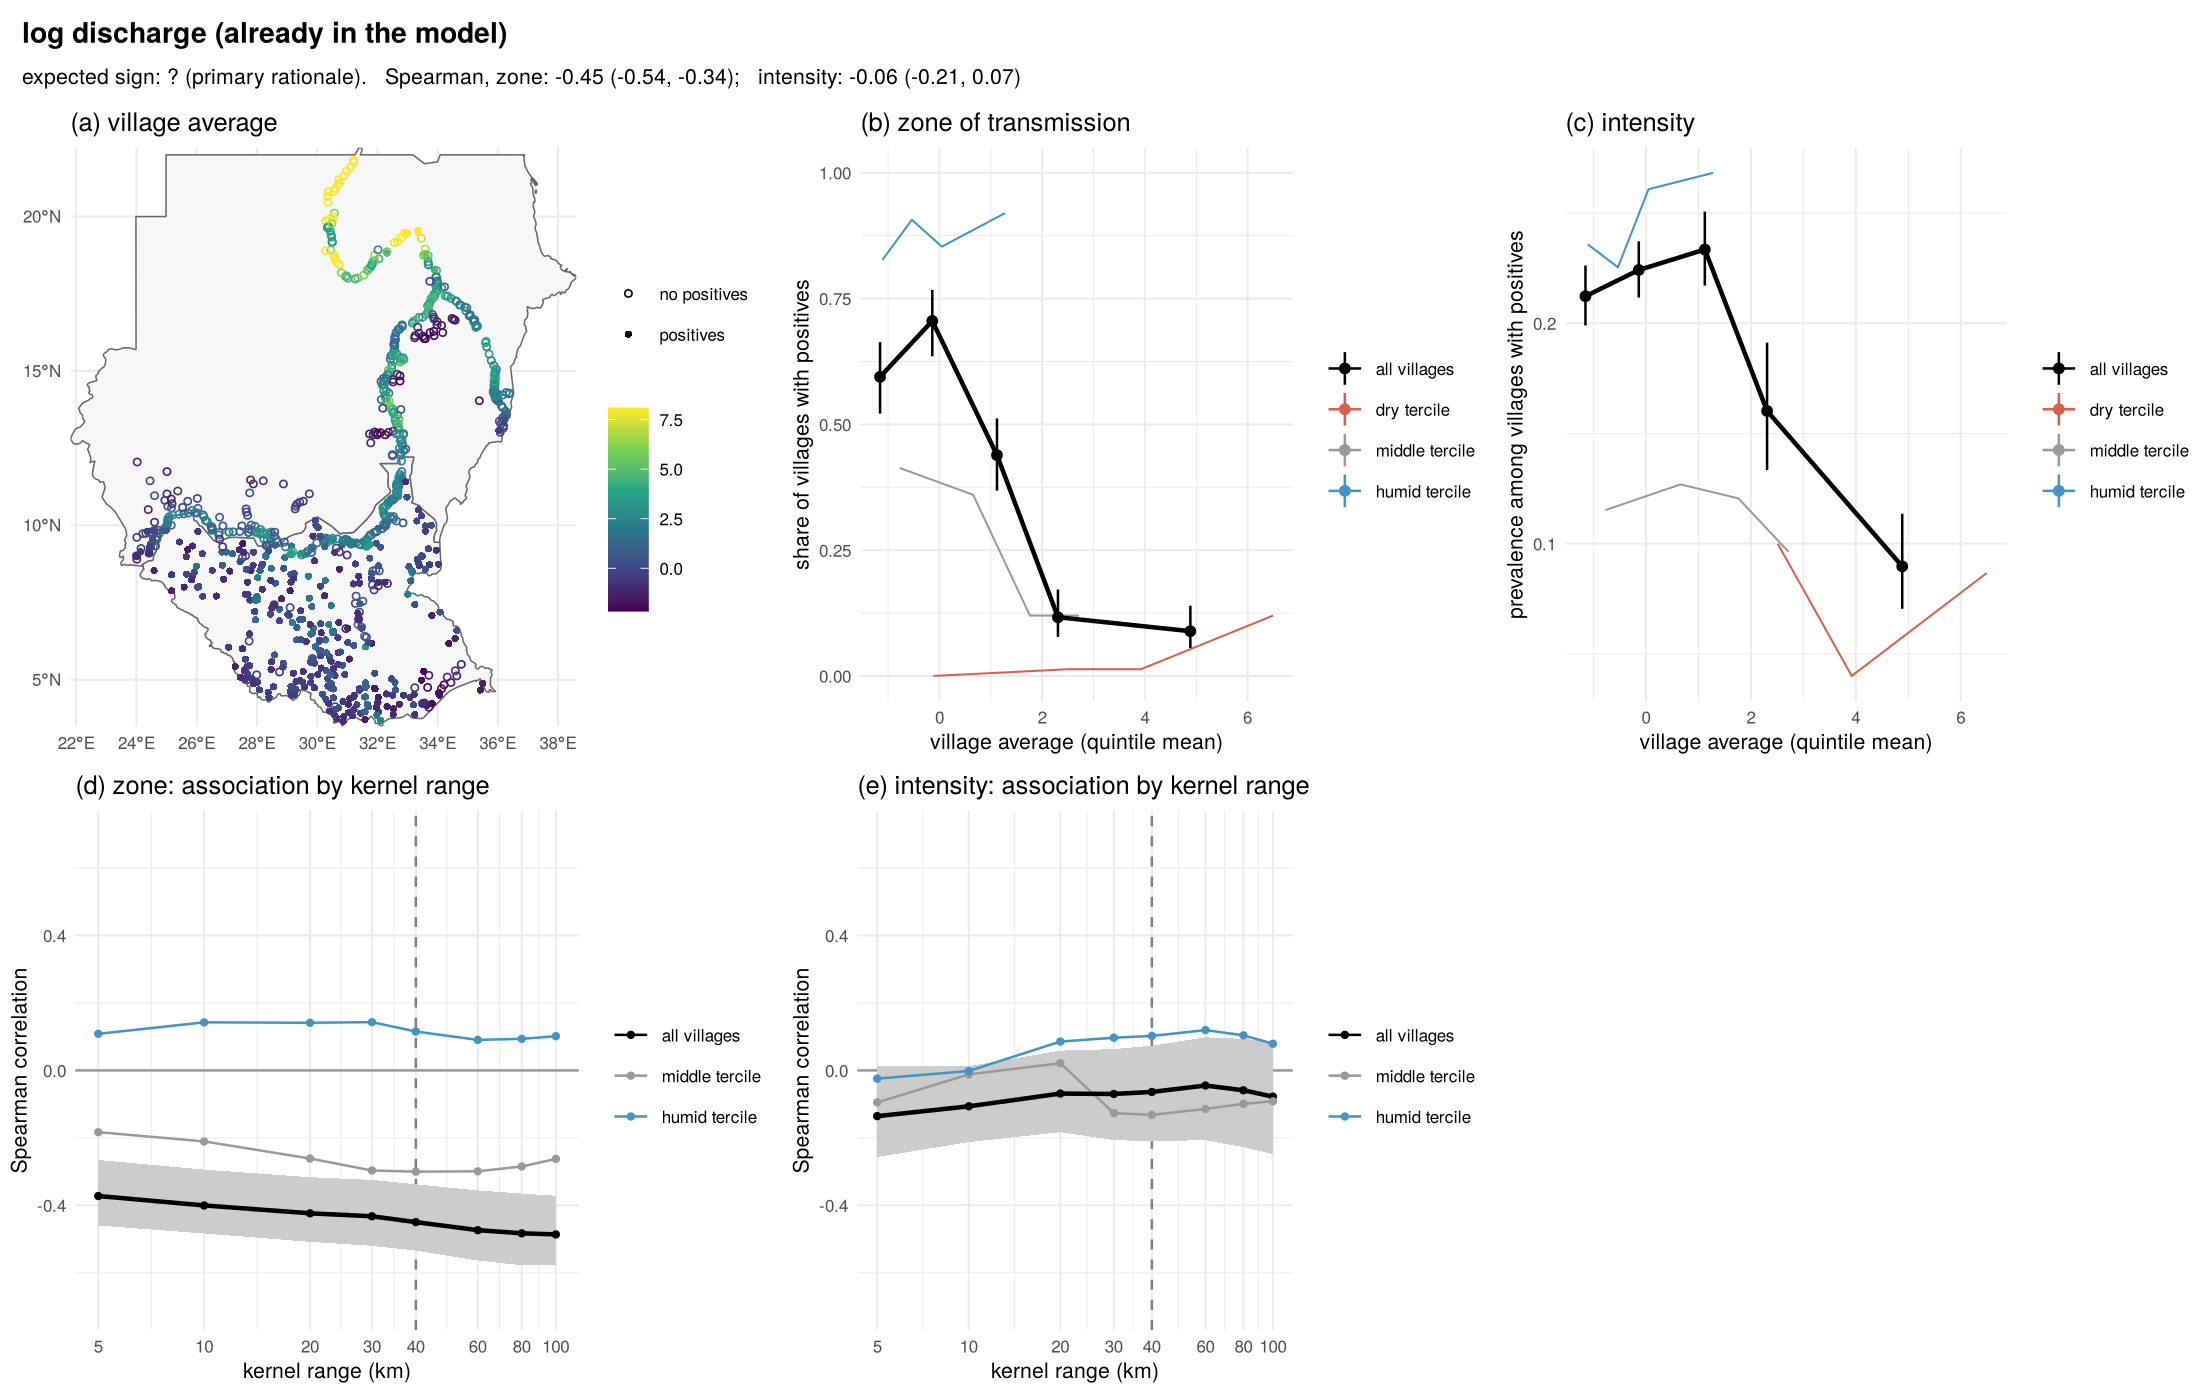
\includegraphics[width=\textwidth]{eda_log_discharge.png}\caption{Log discharge, already in the model. Panels as in Figure~\ref{fig:slope}.}\label{fig:discharge}\end{figure}

\begin{thebibliography}{9}
\bibitem[Crosskey(1990)]{crosskey1990} Crosskey, R. W. (1990). \textit{The Natural History of Blackflies}. Chichester: Wiley.
\bibitem[Hartmann and Moosdorf(2012)]{hartmann2012} Hartmann, J. and Moosdorf, N. (2012). The new global lithological map database GLiM: a representation of rock properties at the Earth surface. \textit{Geochemistry, Geophysics, Geosystems} 13, Q12004.
\bibitem[Linke et al.(2019)]{linke2019} Linke, S., Lehner, B., Ouellet Dallaire, C., Ariwi, J., Grill, G., Anand, M., Beames, P., Burchard-Levine, V., Maxwell, S., Moidu, H., Tan, F. and Thieme, M. (2019). Global hydro-environmental sub-basin and river reach characteristics at high spatial resolution. \textit{Scientific Data} 6, 283.
\end{thebibliography}

\end{document}
